\documentclass[times,english,brazil,oneside, a4paper, fleqn]{ifes8}

\usepackage[utf8]{inputenc}
\usepackage{lastpage}           % Usado pelo exemplo de ficha catalográfica
\usepackage[alf]{abntex2cite}
\usepackage{microtype}          % para melhorias de justificação
\usepackage{morefloats}         % permite mais floats
\usepackage{listings}
\usepackage{xcolor}
\usepackage{tikz}
\usetikzlibrary[topaths]
\usepackage{mathtools}
\usepackage[final]{pdfpages}
%\usepackage{caption}
\usepackage{subcaption}
\usepackage{multirow}
\usepackage{boxhandler}
\usepackage{todonotes}
\usepackage{longtable}
\usepackage{placeins}

\definecolor{dkgreen}{rgb}{0,0.6,0}
\definecolor{gray}{rgb}{0.5,0.5,0.5}
\definecolor{mauve}{rgb}{0.58,0,0.82}

\definecolor{mygreen}{rgb}{0,0.6,0}
\definecolor{mygray}{rgb}{0.5,0.5,0.5}
\definecolor{mymauve}{rgb}{0.58,0,0.82}


%%% The \raggedbottom declaration makes all pages the height of the text on that page.
%%% No extra vertical space is added.
\raggedbottom

%%% Definição da linguagem padrão do documento (pacote babel) para
%%% definir que certas porções do texto (como o resumo, por exemplo)
%%% estão em uma língua estrangeira, usar as macros
%%% \foreignlanguage{languageB}{Text in another language}
%%% ou
%%% \begin{otherlanguage}{languageB}
%%% ...
%%% \end{otherlanguage}
\selectlanguage{brazil}

\setlength{\abovecaptionskip}{5pt} % espaçamento antes da legenda de tabelas/figuras



%%% Define que todos os códigos fontes construídos com o ambiente
%%% `lstlisting' terão uma borda simples.
\lstset{ %
  backgroundcolor=\color{white},   % choose the background color
  basicstyle=\footnotesize,        % size of fonts used for the code
  breaklines=true,                 % automatic line breaking only at whitespace
  captionpos=b,                    % sets the caption-position to bottom
  commentstyle=\color{mygreen},    % comment style
  escapeinside={\%*}{*)},          % if you want to add LaTeX within your code
  keywordstyle=\color{blue},       % keyword style
  stringstyle=\color{mymauve}, 
  numbers=left,
  stepnumber=1,    
  firstnumber=1,
  numberfirstline=true% string literal style,
   frame=top,frame=bottom, frame=single,
   captionpos=t,
   literate=
  {á}{{\'a}}1 {é}{{\'e}}1 {í}{{\'i}}1 {ó}{{\'o}}1 {ú}{{\'u}}1
  {Á}{{\'A}}1 {É}{{\'E}}1 {Í}{{\'I}}1 {Ó}{{\'O}}1 {Ú}{{\'U}}1
  {à}{{\`a}}1 {è}{{\`e}}1 {ì}{{\`i}}1 {ò}{{\`o}}1 {ù}{{\`u}}1
  {À}{{\`A}}1 {È}{{\'E}}1 {Ì}{{\`I}}1 {Ò}{{\`O}}1 {Ù}{{\`U}}1
  {ä}{{\"a}}1 {ë}{{\"e}}1 {ï}{{\"i}}1 {ö}{{\"o}}1 {ü}{{\"u}}1
  {Ä}{{\"A}}1 {Ë}{{\"E}}1 {Ï}{{\"I}}1 {Ö}{{\"O}}1 {Ü}{{\"U}}1
  {â}{{\^a}}1 {ê}{{\^e}}1 {î}{{\^i}}1 {ô}{{\^o}}1 {û}{{\^u}}1
  {Â}{{\^A}}1 {Ê}{{\^E}}1 {Î}{{\^I}}1 {Ô}{{\^O}}1 {Û}{{\^U}}1
  {œ}{{\oe}}1 {Œ}{{\OE}}1 {æ}{{\ae}}1 {Æ}{{\AE}}1 {ß}{{\ss}}1
  {ű}{{\H{u}}}1 {Ű}{{\H{U}}}1 {ő}{{\H{o}}}1 {Ő}{{\H{O}}}1
  {ç}{{\c c}}1 {Ç}{{\c C}}1 {ø}{{\o}}1 {å}{{\r a}}1 {Å}{{\r A}}1
  {€}{{\EUR}}1 {£}{{\pounds}}1
}


\newcommand{\ifestex}{\textsf{Ifes$8$}}

\titulo{Comparação de APIs para Transcrição de Fala na Língua Portuguesa em áudios com Sotaques Regionais Brasileiros}
\autor{Thalles Vargas Ribeiro Lopes}
\autorficha{Lopes, Thalles Vargas}
\local{Serra}
\data{2021}
\orientador[Orientadora:]{Prof.ª Dr.ª Karin Satie Komati}
\coorientador{Prof. Dr. Jefferson Oliveira Andrade}
\instituicao{%
  Instituto Federal do Espírito Santo
}
\curso{Curso Superior de Sistemas de Informação}
\tipotrabalho{Trabalho de Conclusão de Curso}
\preambulo{Trabalho de Conclusão de Curso apresentado à Coordenadoria   do Curso de Sistemas de Informação do Instituto Federal do Espírito   Santo, Campus Serra, como requisito parcial para a obtenção do   título de Bacharel em Sistemas de Informação.}


\begin{document}

\setsecnumformat{\csname the#1\endcsname\space}
\renewcommand{\afterchapternum}{\hspace{-4pt}}

%%% A macro \pretextual não precisa ser explicitamente chamada porque
%%% o abntex2 aciona essa macro no início do documento.
%%% \pretextual

\imprimircapa
%\addtocounter{page}{-1}

\imprimirfolhaderosto*



% Entregue pela Biblioteca
%
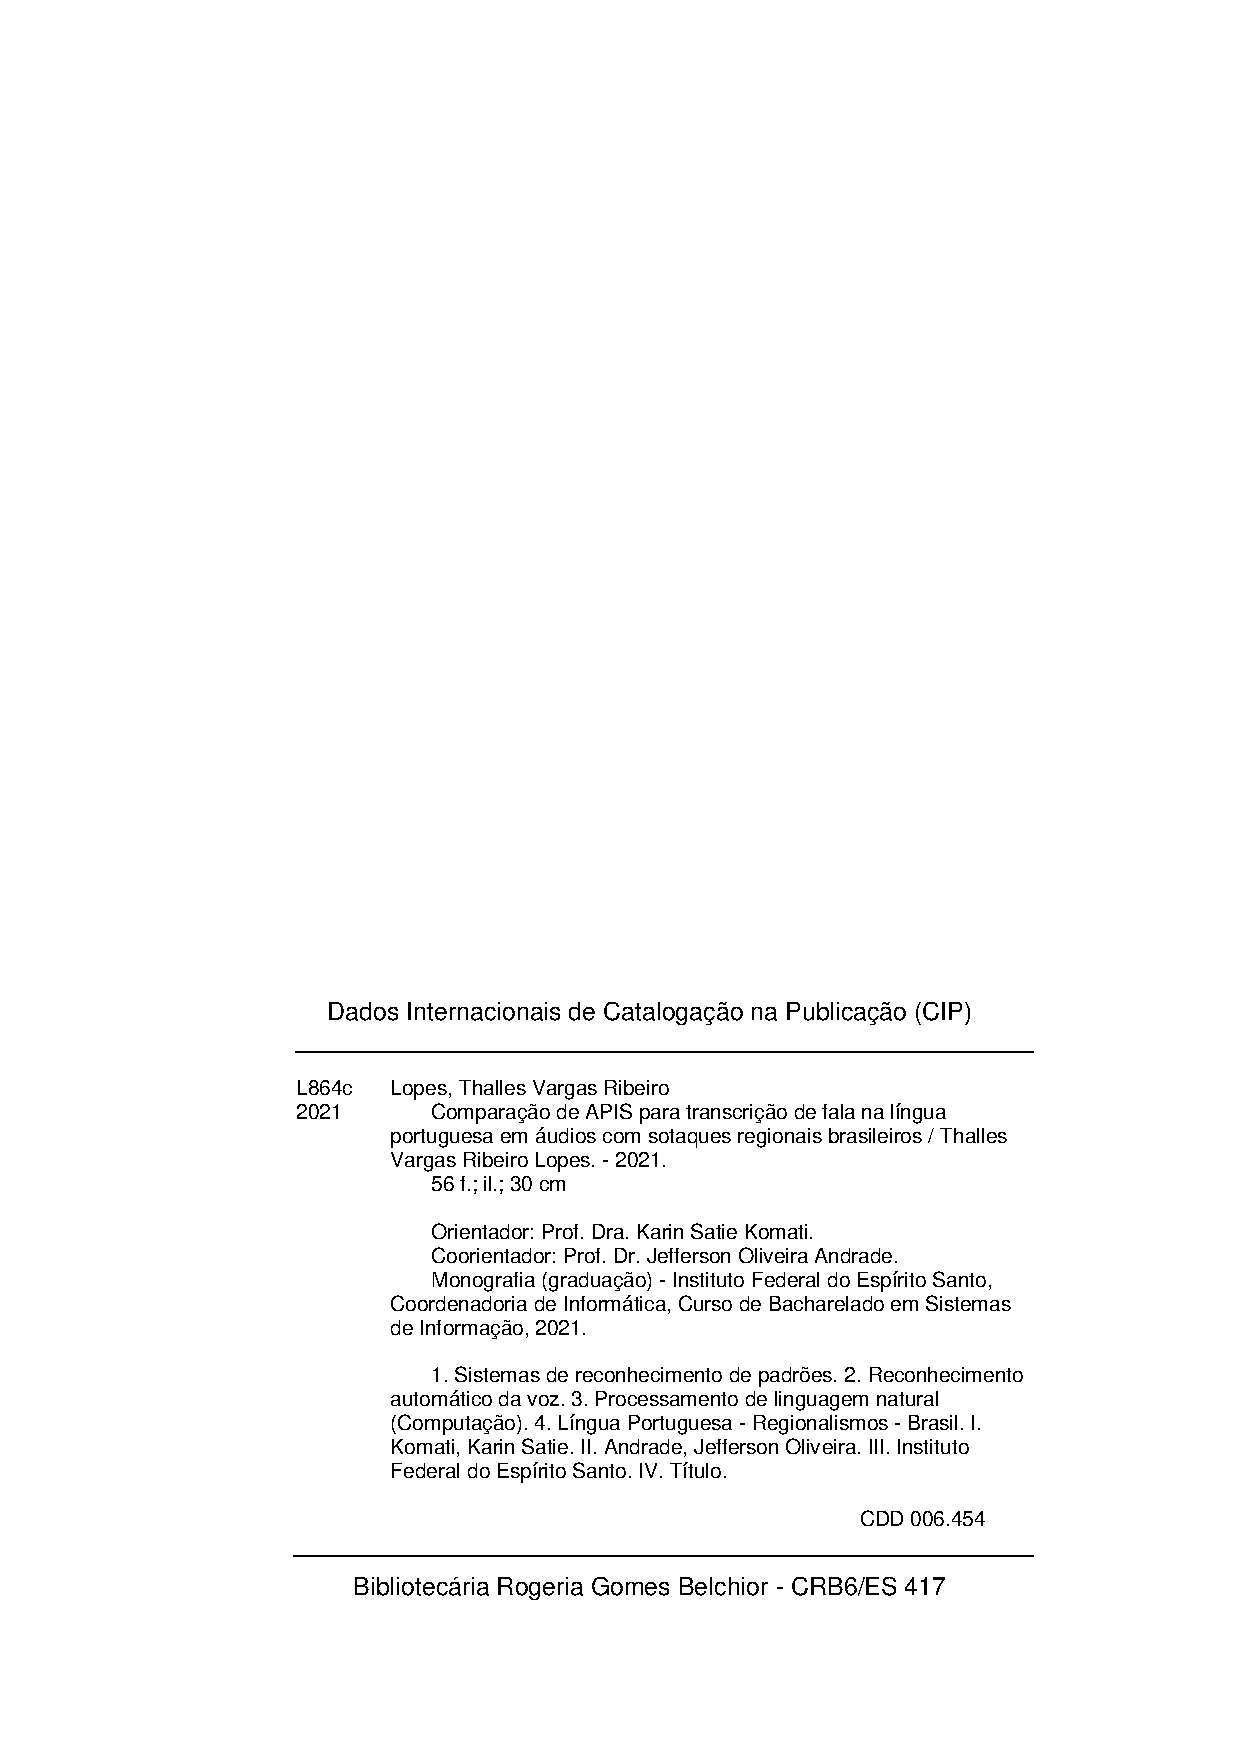
\includepdf{pdf/FichacatalograficaThalles.pdf}
\addtocounter{page}{-1}

%

% ------------------------- Folha de Aprovação ------------------------- 
\newpage



% ------------------------- Folha de Aprovação ------------------------- 
% Entregue pela coordenação
%
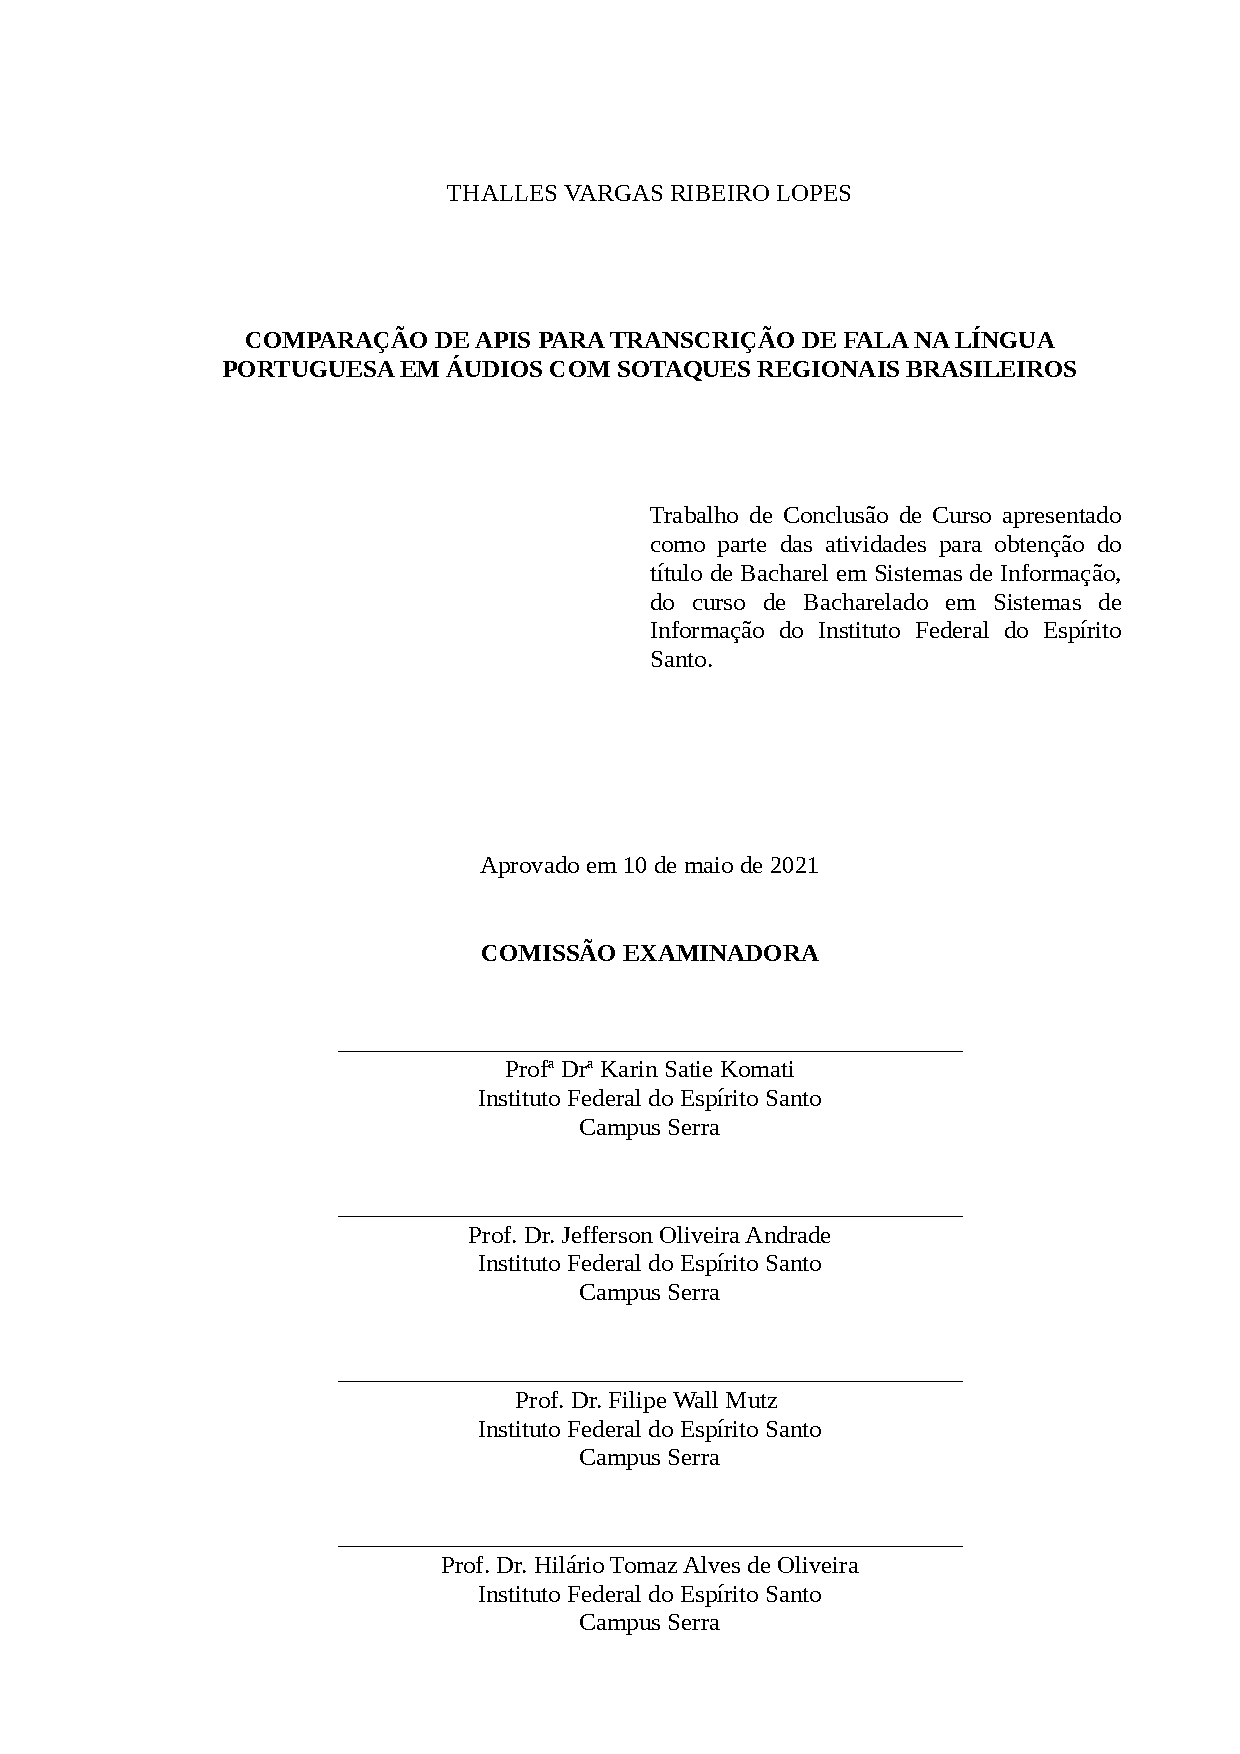
\includepdf[pages=-]{pdf/folha_de_aprovacao_Thalles.pdf}

%%% ====================================================================
%%% Ambiente para a escrita da dedicatória.
\begin{dedicatoria}
  \vspace*{\fill}
 \hspace{0.3\textwidth}
  \begin{minipage}[t][4cm]{0.8\textwidth} 
   \textit{Ao meu pai }  \\
   \textit{À minha mãe }  \\
   \textit{Ao meu irmão }  \\
   \textit{Á minha irmã }  \\
   \textit{À todos aqueles que me acompanharam nessa jornada} 
  \end{minipage}
\end{dedicatoria}


%%% ====================================================================
%%% Agradecimentos
\begin{agradecimentos}
Agradeço a minha família por todo apoio e amor que me deram, por terem me motivado nessa caminhada.

Agradeço a minha orientadora, Prof.a Dr.a Karin Satie Komati e ao meu coorientador prof. Jefferson Andrade, por toda a paciência, dedicação e auxílio.

Por fim, agradeço a todos os colegas e professores que estiveram comigo durante essa jornada no curso.
\end{agradecimentos}





%%% ====================================================================
%%% Epígrafe
%\begin{epigrafe}
%  \vspace*{20cm}
%  \begin{otherlanguage}{english}
%    \begin{flushright}
%      \begin{SingleSpace}%
%		\textit{Power lies where we think it lies} \\ \cite{martin2011clash}
%      \end{SingleSpace}
%    \end{flushright}
  %\end{otherlanguage}
%\end{epigrafe}




%%% ====================================================================
%%% Ambiente para resumo em português
\begin{resumo}[RESUMO]
\vspace*{-6mm}

A tecnologia de transcrição de fala tem evoluído bastante e se tornado mais utilizada devido o crescimento das plataformas de serviço em nuvem. Como existem diversos serviços que entregam essa funcionalidade, surge a dúvida de qual é a mais adequada para processar a língua portuguesa. Neste trabalho, foi realizada uma análise de duas ferramentas de mercado que realizam a transcrição de áudio, com o objetivo de determinar qual a taxa de assertividade de cada uma dessas ferramentas no tratamento de diferentes sotaques brasileiros. 
Para realizar essa comparação foi utilizada a base de dados Braccent que contém uma coleção de áudios que contemplam todas as regiões do Brasil, um conjunto de 1.648 áudios. Foram avaliados fatores regionais, fatores culturais e fatores naturais. Os fatores regionais foram os sete sotaques: nortista, baiano, fluminense, mineiro, carioca, nordestino e sulista; os fatores culturais foi a informação de grau de escolaridade: médio incompleto, médio completo, superior incompleto, superior completo, mestrado e doutorado; e os fatores naturais foi o gênero: masculino e feminino.  Foi realizado a transcrição desses áudios utilizando uma aplicação que fez requisições aos serviços do Google Cloud e Wit.ai. As métricas Levenshtein e Levenshtein Normalizado foram utilizadas para avaliar a taxa de acerto da transcrição da fala. 
Comparando os dados das duas APIs, é possível perceber que a Wit.ai apresenta melhores resultados que o Google Cloud. A média da métrica de Levenshtein Normalizado é de 0,96, enquanto o Google Cloud é de 0,89 considerando símbolos de pontuação. O Wit.ai acertou 81 áudios completos com pontuação. Ressalta-se que sem considerar os símbolos de pontuação, essa quantidade aumenta em 6,7 vezes, acertando 543 áudios. Na análise dos resultados por sotaque, o Google Cloud obteve melhores resultados para o sotaque baiano seguido do nordestino, e os  piores resultados foram para o sotaque carioca e não houve um único acerto para o sotaque nortista. Em todos os sotaques, o Wit.ai apresentou resultados melhores que o Google Cloud. O Wit.ai foi bem em todos os sotaques, apresentando um resultado um pouco pior para o sotaque carioca. 
Os resultados do Google Cloud são melhores para o gênero feminino que o do masculino. Nos resultados do  Wit.ai também, mas a diferença é bem pequena podendo ser  considerada equiparável. Quanto aos resultados por grau de escolaridade, é possível verificar que o nível de ensino não é um fator discriminador para as ferramentas de transcrição considerando a base de dados usada. Ao final, considera-se que o Wit.ai apresentou resultados melhores em todos os cenários, além de transcrever a os símbolos de pontuação.


Palavras-chave: Base de dados Braccent. Fala-para-texto. Google Cloud. Wit.ai. Reconhecimento Automático de Fala.


%A API Wit.ai apresentou melhores resultados em todas as comparações realizadas, além de que o Google Cloud não faz uso de pontuações. Através da metodologia proposta, conclui-se que a Wit.ai possui melhores resultados independente de qualquer característica do locutor (sexo, grau de ensino, região) para transcrições de áudios em PT-BR.

\end{resumo}
    



%%% ====================================================================
%%% Ambiente para resumo em inglês.

\begin{resumo}[ABSTRACT]
\begin{otherlanguage}{english}
\vspace*{-6mm}


Speech transcription technology has evolved a lot and has become more used due to the growth of cloud service platforms. As several services deliver this functionality, it raises the question of which is the most suitable to process the Portuguese language. In this work, an analysis of two market tools that perform audio transcription was carried out, aiming to determine the rate of assertiveness of each of these tools in treating different Brazillian accents. The Braccent database was used to perform this comparasion, which contains a collection of audios that covers all regions of Brazil, a subset of 1,648 audios. It was possible to evaluate regional factors, cultural factors, and natural factors. The regional factors were the seven accents: nortista, baiano, fluminense, mineiro, carioca, nordestino e sulista; the cultural factors were the information on the level of education: incomplete high school, complete high school, incomplete higher education, complete higher education, master's and doctorate; and the natural factors were the gender: male and female. These audios were transcribed using an application that made requests to Google Cloud and Wit.ai services. The Levenshtein and Levenshtein Normalized metrics were used to assess the rate of the correctness of speech transcription. Comparing the data from the two APIs, it is possible to see that Wit.ai presents better results than Google Cloud. The average of the Normalized Levenshtein metric is 0.96, while Google Cloud is 0.89 considering the punctuation. Wit.ai got 81 complete audios with punctuation right. It is noteworthy that without considering the punctuation, this amount increases by 6.7 times, reaching 543 audios. In the analysis of the results by accent, Google Cloud obtained better results for the baiano accent followed by the nordestino, and the worst results were for the carioca accent and there was not a single correct answer for the nortista accent. In all accents, Wit.ai showed better results than Google Cloud. Wit.ai did well in all accents, showing a slightly worse result for the carioca accent. Google Cloud results are better for women than for men. In the Wit.ai results too, but the difference is very small and can be considered comparable. As for the results by level of education, it is possible to verify that the level of education is not a discriminating factor for the transcription tools considering the database used. In the end, it is considered that Wit.ai presented better results in all scenarios, in addition to transcribing the punctuation. 



Keywords: Braccent database. Speech-to-text. Google Cloud. Wit.ai. Automatic Speech Recognition.


  \end{otherlanguage}
\end{resumo}


\renewcommand{\afterloftitle}{\null\\[5mm]}
\renewcommand{\afterlottitle}{\null\\[5mm]}
\renewcommand{\afterloqtitle}{\null\\[5mm]}
\renewcommand{\aftertoctitle}{\null\\[5mm]}


%%% ====================================================================
%%% Lista de figuras
\renewcommand{\listfigurename}{LISTA DE FIGURAS}
\pdfbookmark[0]{\listfigurename}{lof}
\listoffigures*
\cleardoublepage


%%% ====================================================================
%%% Lista de tabelas
%\pdfbookmark[0]{\listtablename}{lot}
%\listoftables*
%\cleardoublepage


%%% ====================================================================
%%% Lista de quadros
\pdfbookmark[0]{\listadequadrosname}{loq}
\listadequadros*
\cleardoublepage


%%% ====================================================================
%%% Lista de abreviaturas
%\begin{abreviaturas}
%  \simb{Abrev.} -- Abreviatura
%  \simb{Assoc.} -- Associação
%  \simb{Atm.} -- Atmosfera
%  \simb{Bel.} -- Bacharel
%  \simb{Bioq.} -- Bioquímica
%  \simb{Cit.} -- Citação
%  \simb{Compl.} -- Complemento
%  \simb{Dic.} -- Dicionário
%  \simb{Dipl.} -- Diploma
%\end{abreviaturas}


%%% ====================================================================
%%% Lista de siglas
%\begin{siglas}
  %\simb{ABNT} -- Associação Brasileira de Normas Técnicas
  %\simb{ACM} -- Association for Computing Machinery
  %\simb{APA} -- American Psychological Association
  %\simb{BIOS} -- Basic Input / Output System
  %\simb{CREA} -- Conselho Regional de Engenharia e Agronomia
  %\simb{IBGE} -- Instituto Brasileiro de Geografia e Estatística
  %\simb{IEEE} -- Institute of Electrical and Electronics Engineers
  %\simb{Ifes} -- Instituo Federal de Educação, Ciência e Tecnologia do Espírito Santo
  %\simb{ISDN} -- Integrated Services Digital Network
  %\simb{RISC} -- Reduced Instruction Set Computer
%\end{siglas}


%%% ====================================================================
%%% Lista de símbolos
%\begin{simbolos}
 % \simb{$\Gamma$} -- Letra grega Gama
  %\simb{$\Lambda$} -- Lambda
  %\simb{$\zeta$} -- Letra grega minúscula zeta
  %\simb{$\in$} -- Pertence
  %\simb{$\top$} -- Valor lógico máximo dentro de um reticulado regular booleano ou quasi-booleano.
%\end{simbolos}
\cleardoublepage


%%% ====================================================================
%%% Sumário --- Table of Contents
\renewcommand{\contentsname}{SUMÁRIO}
\pdfbookmark[0]{\contentsname}{toc}
\tableofcontents*
\cleardoublepage


% ----------------------------------------------------------
% ELEMENTOS TEXTUAIS
% ----------------------------------------------------------
\textual


% ---
% ------------------------ Introdução ------------------------
% ---

\captionsetup{justification=justified,singlelinecheck=false}

%tabulacao para a listagem
%\newcommand{\itab}[1]{\hspace{0em}\rlap{#1}}
%\newcommand{\tab}[1]{\hspace{.2\textwidth}\rlap{#1}}

%inicio do capitulo
\chapter[INTRODUÇÃO]{INTRODUÇÃO}

A capacidade e necessidade de se comunicar surge desde o berço, fruto de educação, podendo ser expressada de várias formas, seja ela escrita ou  oral \cite{falcao2014leitura}. A comunicação é a vantagem evolutiva humana quando comparado com os demais seres que existem, pois através dela é possível trocar informações uns com os outros, possibilitando a elaboração de ideias para sobreviver e enfim dominar o mundo ao seu redor \cite{dos2018importancia}.  

Para permitir que a máquina consiga compreender e reproduzir as formas de comunicação humana, cientistas e engenheiros estudam uma área de
pesquisa de Processamento de Linguagem Natural (NLP, do inglês \textit{Natural language processing}), que envolve várias aplicações, tais como:
\begin{itemize}
    \item Sumarização automática: produz um resumo legível de uma parte do texto. 
    \item Reconhecimento de locutor: identificação da pessoa através da voz \cite{campbell1997speaker}, podendo ser utilizado como mecanismo de segurança em alguns sistemas.
    \item Análise de subjetividade (\textit{sentiment analysis} ou \textit{opinion mining}): Extrai informações subjetivas geralmente de um conjunto de documentos, muitas vezes usando revisões online para determinar a ``polaridade'' sobre objetos específicos. É especialmente útil para identificar tendências da opinião pública nas mídias sociais, para fins de marketing \cite{ding2014sibgrapi}.
    \item Desambiguação: muitas palavras têm mais de um significado, assim temos que selecionar o significado que faz mais sentido no contexto.
    \item Extração de relacionamento: identifica as relações entre entidades nomeadas (por exemplo, quem é casado com quem) com base em textos.
    \item Segmentação morfológica: separa palavras em morfemas individuais e identifica classes de morfemas.
\end{itemize}

Este trabalho versa sobre a aplicação denominada de  Reconhecimento Automático de Fala (ASR, do inglês \textit{Automatic Speech Recognition}) ou também conhecido por sistemas \textit{Speech-To-Text} (literalmente, Fala-para-Texto). O ASR  consiste no processo de conversão de um sinal acústico em um conjunto de palavras que foram ditas  \cite{voiceinteraction}. O primeiro sistema de reconhecimento de fala conhecido e documentado foi construído em 1952 por Davis, Biddulph e Balashek em Bell Laboratories, sistema era capaz de reconhecer dígitos, alcançando precisão de 97-99\% quando era adaptado ao falante \cite{juang2005automatic} \cite{pieraccini2012audrey}. Posteriormente, surgiram diversos usos para o reconhecimento de fala, como ferramenta de interação entre humano e máquina, por exemplo:

    \begin{itemize}
        \item Aplicativos, como Siri, Cortana e Google Assistant, que permitem que o usuário acione funções ou realize buscas através de comandos de voz \cite{lopez2017alexa};
        \item Atendimento ao cliente via de \textit{chatbots} \cite{raju2018contextual}.
        \item Tecnologias Assistivas, como por exemplo em \citeonline{lima2015reconhecimento}, em que é desenvolvido um ambiente virtual para pessoas cegas.
        \item Legendas automáticas de vídeos.
        \end{itemize}


A \autoref{fig:fluxo} ilustra o fluxo do ASR, que se inicia com o usuário falando uma frase ao sistema \cite{cpqd}. A frase corresponde a um sinal de áudio, marcado por um retângulo verde. O sinal de áudio é processado pelo motor de reconhecimento de fala, que converte o áudio para texto. 

\begin{figure}[h!]
\centering
\caption{Fluxo geral do reconhecimento.}
\label{fig:fluxo}
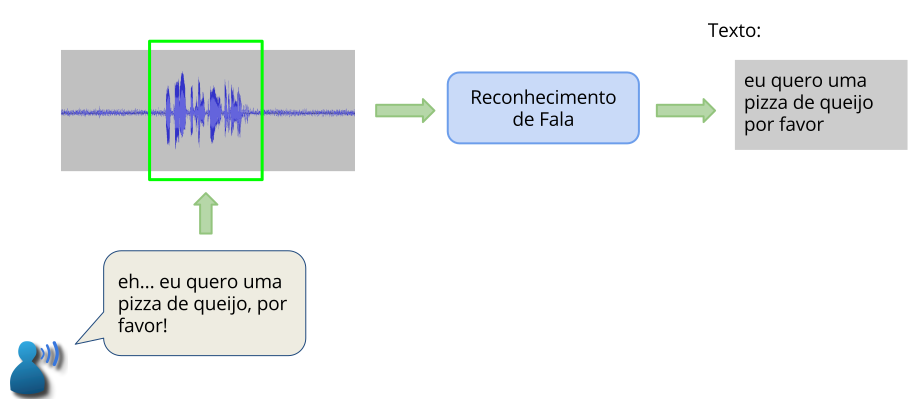
\includegraphics[width=\textwidth]{images/asr-flow.png}
\fonte{\citeonline{cpqd}.}
\end{figure}


%\todo[inline]{DEFINIÇÃO DE TRANSCRIÇÃO, vantagens e aplicações}

%As principais vantagens para o seu uso é a facilidade de registrar informações, realizando o processo de forma automática e muito mais rápida quando comparado com o trabalho manual. Também deve ser notado o benefício de alterar o formato de um vídeo para texto para impulsionar a divulgação, fazendo com que alcance mais pessoas que preferem ler um texto. De forma ainda mais específica na questão "alcançar mais pessoas", é de grande importância na acessibilidade de deficientes auditivos que não conseguiriam compreender o conteúdo do áudio \cite{litero}.

A transcrição da fala pode facilitar e trazer conforto ao dia a dia permitindo abrir aplicativos e digitar textos através da fala  \cite{litero}. Porém seu uso não se limita a isso, atualmente também é utilizado em ambientes corporativos, elevando muito a produtividade de tarefas. Por exemplo, empresas que realizam muitas reuniões, transcrevendo as atas diretamente de áudio para texto, aumentando a produtividade ao automatizar essas tarefas. No campo judiciário também possui grande destaque, uma vez que podem substituir o digitador responsável por documentar toda a sessão em formato de texto, otimizando o tempo e recursos que podem ser alocados para outras tarefas. Além disso, vale ressaltar também o uso em: investigações, escutas telefônicas, gravação de depoimentos, audiências, sessões parlamentares, transcrição de aulas, adaptação de conteúdos para deficientes auditivos,  dentre outros \cite{computerworld}. 

%\section{DIFICULDADES}

%\todo[inline]{dissertação do braccent tem muita informação e referencia interessante}
No exemplo apresentado na \autoref{fig:fluxo}, nota-se que a frase resultante do sistema não é exatamente a mesma, a parte inicial ``eh...'', que indica uma certa hesitação da pessoa não foi convertida, bem como os símbolos de pontuação ',' e '!' também não foram compreendidas pelo sistema. A exclamação tem a ver com entonação da voz da pessoa, e pontuações em geral, ainda é um tema em estudo \cite{zelasko2018punctuation}. Outro tema em estudo é o cenário em que há várias pessoas conversando simultaneamente \cite{sudoh2020simultaneous}. Um fator que pode dificultar o ASR é a qualidade do áudio e o ruído ambiente que podem confundir o sistema \cite{sharan2016overview}. 

\begin{figure}[h!]
\centering
\caption{Mapa de dialetos do português brasileiro}
\label{fig:mapa}
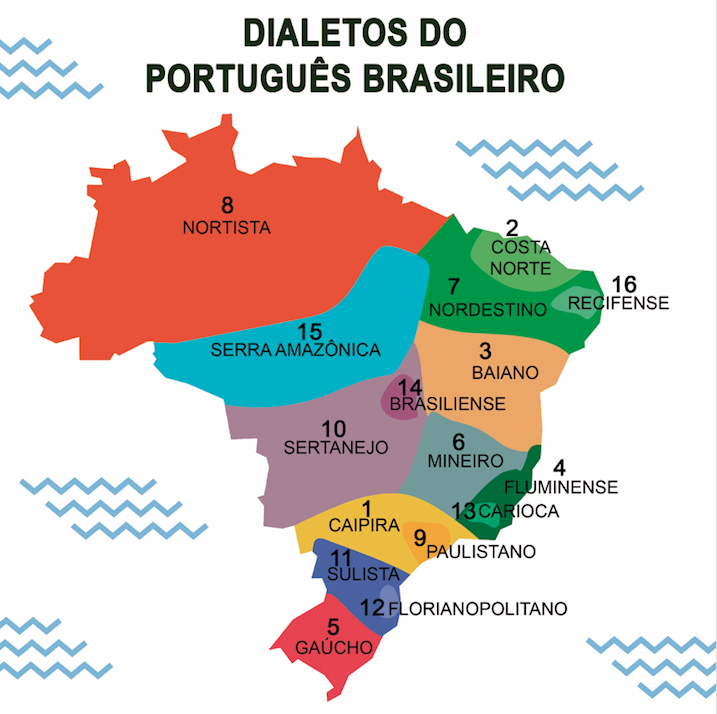
\includegraphics[width=0.5\textwidth]{images/dialeto-portugues.png}
\fonte{\citeonline{dialetoportugues}.}
\end{figure}

Também devemos levar em consideração a língua falada, pois dependendo da língua, os recursos disponíveis variam. A língua inglesa é a que possui mais estudos e por consequência uma maior base de dados, modelos e resultados para trabalhar comparado à língua portuguesa, por exemplo. Outra  questão é que há diferentes sotaques para a mesma língua dependendo da região, como é possível observar no mapa da \autoref{fig:mapa}, que apresenta uma divisão do território brasileiro por sotaque. Cada sotaque pode ter uma diferente pronúncia para algumas palavras, o que pode confundir o sistema de reconhecimento de fala \cite{viglino2019end}. 
%Por esses motivos o reconhecimento de fala processando a língua portuguesa acaba obtendo uma menor taxa de acertabilidade quando comparado ao inglês \cite{alvarenga2019transcriccao}.

 %\cite{waibel1990readings}
 %e o tamanho do vocabulário pode aumentar a complexidade caso seja muito grande.
%não possui em domínio público um sistema de reconhecimento automático de voz para o português, com suporte a grandes vocabulários. 

\section{A PROPOSTA}


A proposta deste trabalho é comparar Applications Programming Interface (API),  que tem o serviço de ASR para a língua portuguesa, em uma base de dados com sotaques regionais brasileiros distintos. 
Ha várias APIs no mercado, a página \citeonline{listaAPI} contém uma lista das 10 que o autor considera as melhores do mercado. As APIs foram selecionadas levando em consideração se são renomadas ou não e quais processam a língua portuguesa (pt-BR). 
Outra quesito que foi considerada é o custo de sua utilização. A fim de reduzir o custo do desenvolvimento do trabalho, todas as APIs devem ser gratuitas ou disponibilizem de forma gratuita por um quantidade pré-definida de período/uso. Ao final, foram selecionadas duas APIs: Google Cloud Speech API\footnote{https://cloud.google.com/speech-to-text} e Wit.ai\footnote{https://wit.ai/}. 
%Já sabemos que para o inglês apresenta ótimos resultados, uma vez que as primeiras aplicações foram feitas baseadas na língua, o que justifica um maior desenvolvimento para ela.

Como fonte de dados foi utilizado a base de dados Braccent, criada por \citeonline{batista2019estudo}, que é uma base de áudios com grande diversidade de sotaques. Foi usado um subconjunto de 1.648 áudios da base de dados Braccent. As gravações são identificadas de acordo com o gênero e o sotaque regional falado na locução, sendo 854 amostras do sexo feminino e 794 amostras do sexo masculino. Os sotaques são: nortista, baiano, fluminense, mineiro, carioca, nordestino e sulista. Além da informação do sotaque, há ainda a informação de grau de escolaridade: médio incompleto, médio completo, superior incompleto, superior completo, mestrado e doutorado. Assim, será possível comparar os resultados por fatores regionais, culturais e naturais  \cite{correiacomunicaccao}: 

\begin{itemize}
    \item Fatores regionais: é a diferença do português falado por uma pessoa nascida e criada na região nordeste e outro na região sul do Brasil. 
    \item Fatores culturais: o grau de escolarização e a formação cultural de uma pessoa são fatores que podem soar diferentemente aos ouvidos de outra pessoa. 
    \item Fatores naturais: o uso da língua pelos falantes sofre influência de fatores naturais, como idade e sexo. Uma criança não fala da mesma forma que um adulto.
\end{itemize}


A escolha dessa base foi feita justamente para analisar o comportamento destas APIs quando utilizadas para processar toda a variedade do pt-BR. A \autoref{diagramaAPIintro} apresenta a arquitetura geral do ambiente de testes desenvolvido usando a linguagem de programação Python que usará as duas API para transcrição dos áudios da base de dados Braccent. Para analisar a taxa de acerto da transcrição da fala foram utilizadas as métricas Levenshtein e  Levenshtein Normalizado. 

\begin{figure}[h!]
\centering
\caption{Modelo de funcionamento.\label{diagramaAPIintro}}
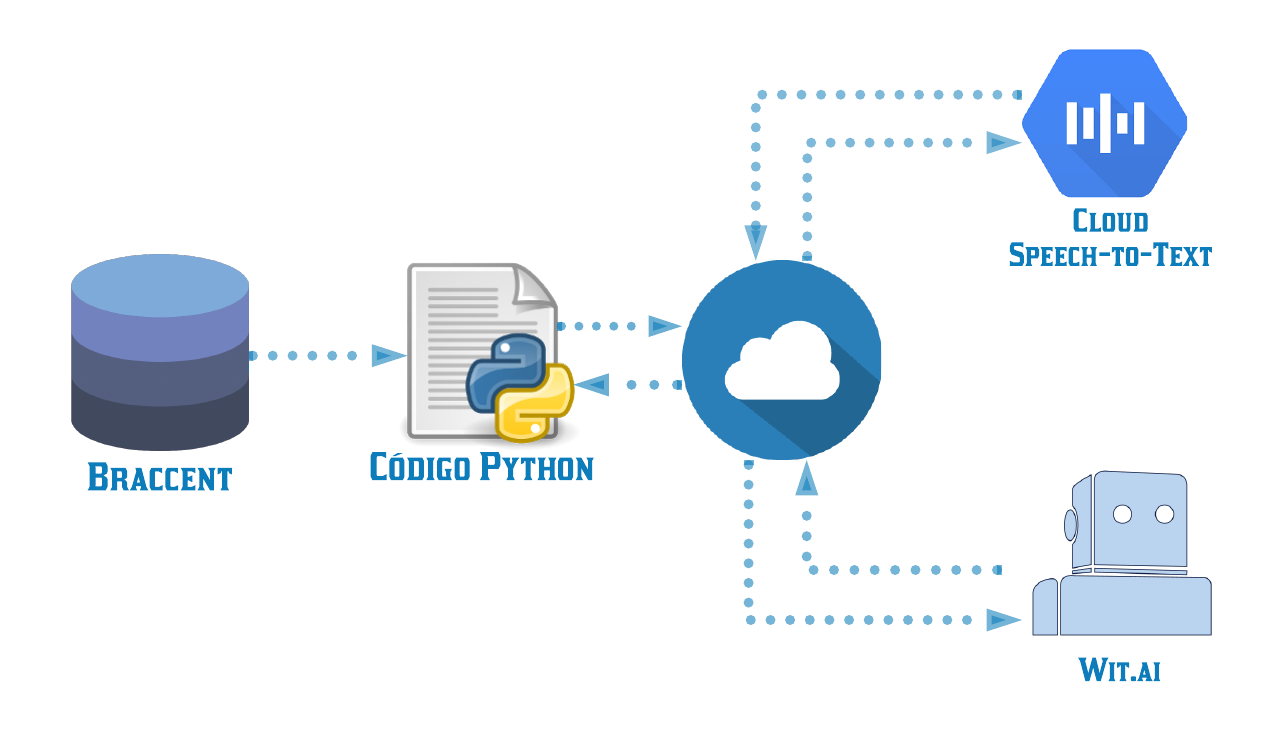
\includegraphics[width=115mm]{images/Diagramas/APIs.png}
\fonte{elaborado pelo próprio autor (2021)}
\end{figure}


%\todo[inline]{Terminar de escrever a parte de métricas de erro após a finalização do cap4}
%para analisar a taxa de acerto da transcrição da fala através da métrica WER, coletando os áudios para teste da base de dados Braccent.
%No processo de transcrição algumas palavras podem ser transcritas de forma errada, para calcular taxa de erros de uma transcrição, 

%uma métrica utilizada para mensurar a precisão de aplicações de ASR denominada Word Error Rate (WER), sendo basicamente a soma do número de palavras substituídas, inseridas e deletadas dividido pelo número de palavras totais \cite{wer}.

%\begin{itemize}
    %\item palavras substituídas: uma palavra é substituída por outra, por exemplo: trocar comprimento por cumprimento;
    %\item palavras inseridas: uma palavra que não foi dita é incluída no texto transcrito, por exemplo:
    %\item palavras deletadas: uma palavra que foi dita porém não foi incluída no texto transcrito, por exemplo: "jogue isso assim" vire "jogue assim".
%\end{itemize}


\section{OBJETIVOS}
\subsection{Objetivo Geral}

O objetivo deste trabalho é comparar a taxa de acerto da transcrição da fala em língua portuguesa, levando em consideração diferentes sotaques regionais brasileiros, graus de escolaridade e gêneros, das ferramentas Google Cloud e Wit.ai.

\subsection{Objetivos Específicos}

Os objetivos específicos identificados para se atingir o objetivo geral proposto são:
\begin{itemize}
    \item Pesquisar sobre as APIs, Google Speech API e  Wit.ai.
    \item Pesquisar sobre as métricas de comparação de \textit{strings}.
    \item Desenvolver ambiente dos experimentos, com coleta de dados e estatísticas.
\end{itemize}


%\section{LIMITAÇÕES}

\section{ESTRUTURA DO TEXTO}

Este trabalho está dividido em cinco capítulos. Este primeiro capítulo trouxe uma introdução ao problema estudado, a contextualização do tema, a justificativa para a sua realização e os objetivos pretendidos.  O Capítulo 2 apresenta detalhes da base de dados Braccent e das ferramentas Google Speech API e  Wit.ai, além do detalhamento da métrica de Levenshtein. Em seguida, o Capítulo 3 traz o desenvolvimento do sistema e o Capítulo 4 traz os resultados dos áudios processados e a discussão associada. Por fim, no Capítulo 5, são tecidas as considerações finais e os trabalhos futuros.

\begin{comment}
Por conta da tecnologia existente na época, os resultados não eram tão significativos, o que fazia com que o Reconhecimento de Fala não tivesse tanta visibilidade. Porém por causa de diversos motivos ligados ao avanço tecnológico da humanidade estamos tendo cada vez mais contato com ASR. \citeonline{yu2016automatic} citam 3 fatores para estarem ocorrendo essas mudanças, elas são:

\begin{itemize}
    \item O poder computacional que está disponível;
    \item O avanço da internet contribuindo com a quantidade de acesso a mais dados;
    \item O uso cada vez maior de dispositivos portáteis (\textit{smartphones}, \textit{smartwatches}, dentre outros).
\end{itemize}

   
%Todos esses vários usos  do Reconhecimento de Fala possuem obstáculos em comum que dificultam a sua implementação. 

%Comumente estamos habituados a falar conectando as palavras uma nas outras, essa é a principal característica que pode dificultar o ASR, pois se torna mais difícil de determinar onde uma palavra termina e começa outra. 
%, um problema cujo impacto está diminuindo já que hoje em dia temos a nossa disposição ferramentas melhores para realizar a gravação de áudio. O que também pode afetar a qualidade do áudio que independente do hardware que está sendo utilizado para gravar aplicação com ruídos paralelos caso a gravação não esteja ocorrendo em um local com um nível de silêncio aceitável
\end{comment}

% ---
% ------------------------ Referencial Teórico ------------------------
% ---

\chapter[REFERENCIAL TEÓRICO]{REFERENCIAL TEÓRICO}
\index{Referencial Teórico}
%\vspace*{-17mm}

Neste capítulo serão apresentados conceitos gerais do reconhecimento óptico de caracteres, bem como um pouco sobre cada uma das ferramentas usadas neste trabalho, em seguida serão detalhadas as características da base de áudios Braccent e ao final, há a descrição das métricas de comparação dos resultados.


\section{SISTEMAS DE TRANSCRIÇÃO}

Sistemas de transcrição da fala permitem que o computador interprete sinais de áudio, gerando transcrições textuais. 
De acordo com \citeonline{ferreira2017uso}, as arquiteturas clássicas de sistemas de transcrição tem quatro grandes componentes: modelo acústico, o modelo de linguagem, modelo léxico e decodificador. 

\begin{figure}[h!]
\centering
\caption{Arquitetura clássica de ASR.}
\label{fig:arqclassica}
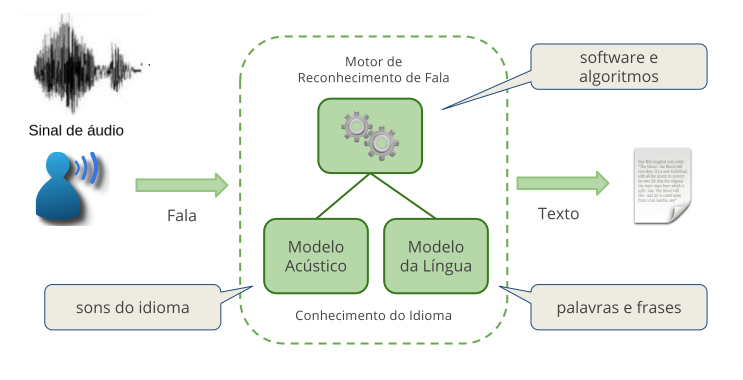
\includegraphics[width=130mm]{images/asr_2.png}
\fonte{\citeonline{cpqd}.}
\end{figure}

A \autoref{fig:arqclassica} apresenta a arquitetura com os componentes, onde o Modelo Acústico mapeia o sinal original que está sendo processado em palavras e sentenças; o Modelo da Língua é responsável por caracterizar a língua, a combinação de palavras e representa as palavras do dicionário com suas transcrições fonéticas; e Motor de Reconhecimento de Fala que é o  decodificador, que procura a melhor sequência de palavras possível. 



%Crescimento que provavelmente também foi impulsionado pela ``democratização da tecnologia'', através do livre acesso à essas tecnologias avançadas disponibilizadas pelos seus desenvolvedores
%O acesso é geralmente disponibilizado através de rotinas e padrões de programação, popularmente denominadas pela sigla API (\textit{Application Programming Interface}).  não passar pelo \textit{firewall}  da empresa,  endereço IP disponibilizado  via  DHCP por VM IP Static/global também estão disponíveis mas com custos adicionais),  Round-robin DNS para load balancing,, distribuição de carga geográfica (exemplo: Big-IP global traffic manager)

Na última década, as técnicas de aprendizado profundo começaram a ser utilizadas com sucesso em ASR \cite{dahl2011context}. Desde então, diversos sistemas comerciais começaram a se popularizar, principalmente os sistemas em nuvem. Devido a capacidade de escalabilidade e abstração, plataformas como serviço tem crescido praticamente 20\% ao ano \cite{krancher2018key}. 
A utilização destas ferramentas trazem vantagens, tais  como: elasticidade (rápida capacidade de escalabilidade), otimização de custos (devido ao compartilhamento de recursos),  virtualização  (fácil alocação  de  recursos), funcionalidades de operação e gestão, diferentes níveis de contratação,  VLANs privadas, controle de acesso dos endereços de IP e  compressão de conteúdo \cite{munteanumeeting}.
Grandes empresas da área tecnológica como IBM, Google, Microsoft, Amazon e Facebook já disponibilizaram serviços que utilizam inteligência artificial, sendo um deles o de transcrição. 

%conversor de voz para texto em que a inteligência artificial é utilizada para combinar as estruturas da linguagem e gramática com o processamento de sinais de voz, afim de obter uma identificação mais precisa das palavras. , fornecendo para diversos empreendimentos alta performance, segurança e confiabilidade em seus processos, otimizando a qualidade dos resultados adquiridos.

As ferramentas selecionadas para o desenvolvimento deste trabalho foram os das empresas Google e Facebook. 
A Google Cloud é uma plataforma mantida pelo Google, com  uma série de serviços na computação em nuvem, utilizado também pela própria empresa em produtos fornecidos ao usuário, como o Youtube. Diversos produtos são disponibilizados através dela, dentre eles podemos citar: processamento através de máquinas, armazenamento de objetos, serviço de banco de dados, processamento visual,  reconhecimento de fala e transcrição \cite{GoogleCloudGeral}. O serviço Speech-to-Text foi utilizado para realizar as transcrições dos áudios, onde uma rede neural é usada para o modelo de reconhecimento de voz com suporte a mais de 120 linguagens e dialetos. Apesar da utilização em geral ser paga, a plataforma fornece créditos válidos por um ano para iniciar o uso. \cite{kimura2018comparison}. 

%\subsection{Wit.ai}
A Wit.ai é mantida pelo Facebook e oferece aos desenvolvedores uma plataforma de linguagem natural que aprende a linguagem humana a partir de cada interação \cite{mitrevski2018getting}. Ao contrário da Google Cloud que é uma plataforma com diversas funcionalidades, a Wit.ai fornece apenas serviço de reconhecimento de fala e texto, sendo muito utilizada para a criação de \textit{chatbot} e reconhecimento da voz em aplicações. 

Para utilização é necessário realizar o login com uma conta do Facebook e não possui planos de uso, sendo totalmente gratuito com suporte para 132 linguagens e dialetos, porém uma de suas limitações é seu limite de tamanho de áudio, atualmente sendo de 20 segundos. Neste trabalho essa limitação não foi um problema, pois todos os áudios da base de dados possuem uma duração menor que o limite, com exceções de áudios que tiveram erros de gravação que foram removidos do escopo. \cite{WIT}.

\section{TRABALHOS CORRELATOS}

Nesta seção detalhamos dois artigos, um artigo de \citeonline{iinumaspeech} que faz uma comparação entre ferramentas da IBM, Google e Amazon para conversão de voz para texto de ligações telefônicas e um segundo artigo de  \citeonline{zelasko2018punctuation} que avalia a pontuação de transcrições de chamadas telefônicas.


Segundo \citeonline{iinumaspeech}, as tecnologias, ``Plataformas como serviço'', ``infraestrutura como serviço'' e ``Inteligência Artificial'',  estão sendo utilizadas para desenvolver sistemas que substituem pessoas em \textit{call centers}. Existindo casos até de fechamento completo de um \textit{call center} para trocar por uma \textit{startup} que utiliza programas de computador que substituem os seres humanos.
No artigo \cite{iinumaspeech} foram comparadas as ferramentas Google Cloud Speech to Text, IBM Watson Speech to Text e Amazon Transcribe. 

A base de dados foi composta de gravações de áudio com 6 (seis) diferentes interlocutores brasileiros que realizaram a leitura de uma parte do livro ``Divina Comédia''. São 3 (três) pessoas do sexo feminino e 3 (três) masculinos. Todos têm titulação de pós-graduação e faixa etária entre 40 e 50 anos. Foram realizados os seguintes pré-processamentos usando o aplicativo Audacity\footnote{https://www.audacityteam.org/}: eliminação de excesso de período sem falas, melhoria do volume e retirada de ruídos. 

%realizado uma pesquisa entre empresas influentes no âmbito tecnológico que disponibilizam serviços que utilizam inteligência artificial, sendo elas . Testando as suas ferramentas de conversão de voz para texto, 
Afim de comparar qual possui a melhor eficiência, foi usada a métrica de Taxa de Erros das Palavras (WER, do inglês \textit{Word Error Rate}). Para o WER, quanto menor o número, melhor será a qualidade do texto obtido. O WER é derivado da distância de Levenshtein, trabalhando no nível da palavra ao invés do nível do fonema. A partir da análise dos dados gerados pelo WER, constataram uma maior eficiência de conversão da API do Google (14,9\%), seguido pela API da IBM (15,23\%) e por último a API da Amazon (16,5\%), nota-se que a diferença entre as taxas de erro é baixa. É importante ressaltar que a pesquisa foi exploratória e as conclusões foram feitas com uma pequena base de experimentos (18 gravações no total) e uma pequena amostra de pessoas (6 pessoas).


% Em teoria, qualquer fonte de texto como blogs, artigos e Wikipédia poderiam ser utilizados como base de dados para realizar o treinamento da aplicação no uso de pontuação, porém a maioria deles não representam a linguagem coloquial. Portanto não dados fáceis de ser encontrados. 
%As redes neurais são treinadas na incorporação Common Web Crawl GloVe das palavras nas transcrições de Fisher alinhadas com os indicadores de conversação e informações de tempo de palavra. 

Em \citeonline{zelasko2018punctuation}, apresenta o problema de que muitos ASR não preveem pontuação ou capitalização. A falta de pontuação pode confundir tanto o leitor humano quanto os algoritmos de processamento de linguagem natural que usarão estes resultados. O texto sem pontuação além de poder ser confuso, pode ser difícil de ler, e algumas vezes perderem o real sentido do que foi dito. 
A proposta do trabalho foi o de treinar duas variantes de modelos de Rede Neural Profunda (DNN, do inglês \textit{Deep Neural Network}): a Memória de Curto-Prazo Longa Bidirecional (BLSTM, do inglês \textit{Bidirectional Long Short-Term Memory}) e uma Rede Neural Convolucional (CNN, do inglês \textit{Convolutional Neural Network}), para a predição de pontuação. 


Os modelos foram treinados no corpus inglês de Fisher \cite{cieri2004fisher}, que contém cerca de 11.000 conversas distintas com  anotações de pontuação. Foram considerados o tempo e duração de cada palavra, solução que até então não havia sido utilizado em outro sistema para realizar a tarefa de predição de pontuação. Nos experimentos, as transcrições de corpus de Fisher são alinhadas no tempo e pontuadas usando um algoritmo de alinhamento de sequência. Foram usadas 4 (quatro) classes de pontuação: espaço em branco (79,1\%), vírgula (11,5\%), ponto final (8,2\%) e ponto de interrogação (1,2\%). Os resultados são apresentados na \autoref{fig:pontos}.



A melhor acurácia foi com o modelo BLSTM considerando o alinhamento com o tempo das palavras. Pela matriz de confusão, o acerto do espaço (\textit{blank}) foi alta (0,95), mas não tanto para as demais pontuações. A CNN foi a que teve mais acertos nos caso de pontos de interrogação. As CNNs apresentam melhor precisão e os BLSTMs tendem a ter uma melhor revocação.  Os resultados constituem evidências significativas de que a distribuição de palavras no tempo podem ser úteis na tarefa de previsão de pontuação, pois apresentaram melhor resultado do que os modelos sem esta característica.


\begin{figure}[h!]
\centering
\caption{Matriz de confusão do melhor modelo BLSTM alinhado no tempo.}
\label{fig:pontos}
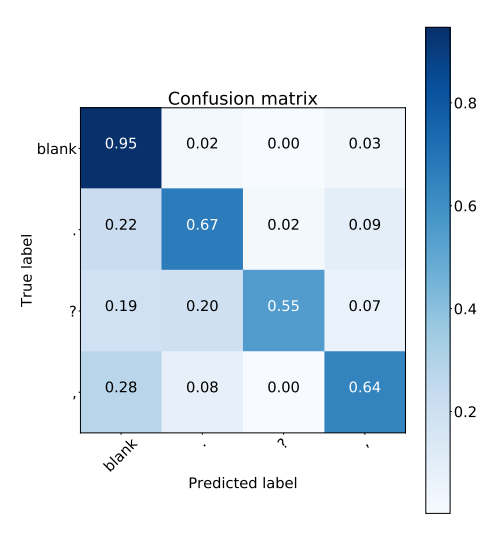
\includegraphics[width=0.5\textwidth]{images/matrzi.png}
\fonte{\citeonline{zelasko2018punctuation}.}
\end{figure}
%s cometam uma quantidade menor de erros no geral, a pontuação prevista pela CNN é mais precisa - especialmente no caso de pontos de interrogação. 

\section{BASE DE DADOS BRACCENT}

A base de dados Braccent foi criada por \citeonline{batista2019estudo}, e contém 1.743 amostras de fala. Há 7 sotaques brasileiros existentes na base, que são: nortista, baiano, fluminense, mineiro, carioca, nordestino e sulista. Os voluntários leem 16 sequências de frases, que foram criadas de forma a serem foneticamente balanceadas em seu conjunto e não necessariamente apresentam uma coerência semântica. O trabalho de origem da base de dados apresenta a  transcrição fonética, que foi realizada manualmente para cada sotaque regional pelos alunos do curso de Letras do ano de 2018 do Instituto de Estudos da Linguagem na Universidade Estadual de Campinas. O balanceamento fonético foi feito via análise da correlação de Spearman com a base Braccent e o CETENFolha\footnote{CETENFolha (Corpus de Extractos de Textos Eletrônicos NILC/Folha de S. Paulo) é um corpus de cerca de 24 milhões de palavras em português brasileiro, criado pelo projeto Processamento computacional do português com base nos textos do jornal Folha de São Paulo que fazem parte do corpus NILC/São Carlos, compilado pelo Núcleo Interinstitucional de Linguística Computacional (NILC).}, que foi de 89\%, maior que os 80\% do limiar descrito na literatura. Seguem as frases, com a pontuação e acentuação tal qual apresentado no trabalho original:

\begin{enumerate}[itemsep=3pt,parsep=3pt]
    \item Eu rasguei todo meu dinheiro em vão, minha família depende da aposentadoria do meu avô. Mas o dia amanheceu ensolarado e eu fiquei feliz porque minha tia viajou para Porto Alegre às sete horas.
    \item O telejornal da Globo terminou agora a pouco, todos se levantaram, a porta bateu forte e meu tio xingou bastante. Mas disse que é um grande prazer ter os sobrinhos hospedados em casa e não em um dos hotéis do sudoeste.
    \item Para ganhar, preciso decifrar o código até amanhã. Os papeis foram rasgados mas ainda é possível ler informações importantes.
    \item Suas atitudes são muito drásticas e resultarão em guerra entre vocês. Ela chegou a pedir o divórcio antes dele morrer e pensou que podia compartilhar esse documento com você.
    \item Meu orientador disse que o professor de Português e a professora de Matemática se casaram e foram morar na Nigéria, onde o clima está muito diferente de dez anos atrás.
    \item Você tem razão, a correção da prova não foi justa e a turma tirou notas abaixo da média. Assim como a gestão do atual prefeito, a diretoria não está agradando o povo.
    \item Tenho aptidão para tirar fotos de motos e guitarras, então recebi em dólar e comprei um carro, jóias e relógios para nós. A atriz teve uma ótima atuação no espetáculo e recebeu meus parabéns e um presente pela apresentação fantástica.
    \item Eu criei muita expectativa nesse trabalho. O chefe não ouviu meu clamor, continuou sorrindo para mim e segurando a colher que estava suja de abacate ele disse ``A palavra caçador se escreve com C cedilha''.
    \item O Brasil é um país injusto e desigual, é errado não partilhar a comida com os mais necessitados. Mas só vota quem tiver o título de eleitor.
    \item Esse canal tem bastante pornografia e a abertura do campeonato ocorreu antes de ontem, quando os turistas japoneses procuravam belas casas para alugar.
    \item O biscoito era de chocolate com morango, por isso escolhi o bombom de chocolate ao leite com licor de Amarula. Ainda precisamos comprar pó de café, pão francês, abóbora e melão.
    \item Segurei a panela de macarrão com apenas uma mão e as duas pilhas que eu lhe dei caíram no chão. A rã está embaixo do fogão, deve ser retirada logo, pois tenho medo de répteis e de minhocas.
    \item Ele pulou daquele caminhão que transportava tubos de ferro e nega que naquela área tem produtos tóxicos. Foi na cidade em que encontraram o corpo do mendigo numa bocada e montaram uma emboscada para prender os assaltantes. 
    \item Ele ficou chateado porque foi chamado de burro pelo escrivão zangado enquanto lavava sua blusa azul de lã com água e sabão.
    \item Li que o escrivão mora sozinho perto da plantação de feijão e sorte que o jacaré que fugiu do zoológico já foi encontrado.
    \item A velha locomotiva vem com pouca carga e os faróis iluminam as flores da rua em que a criança desenhou um vulcão.
\end{enumerate}


As gravações são identificadas de acordo com o gênero e o sotaque regional falado na locução, sendo 872 amostras do sexo feminino e 871 amostras do sexo masculino, conforme distribuição da Tabela \ref{tab:tabBraccent}. É possível verificar pela tabela que há desbalanceamento quanto à quantidade de áudios por sotaque, com muito mais exemplares do sulista enquanto há poucos nortistas.  Foram 142 locutores com diferentes faixas etárias e níveis de escolaridade, e a quantidade de áudio de cada locutor variou entre 1 e 16. 

\begin{table}[h!]
\centering
\caption{Descrição do Número de Gravações da Base de Dados Braccent.}
\label{tab:tabBraccent}
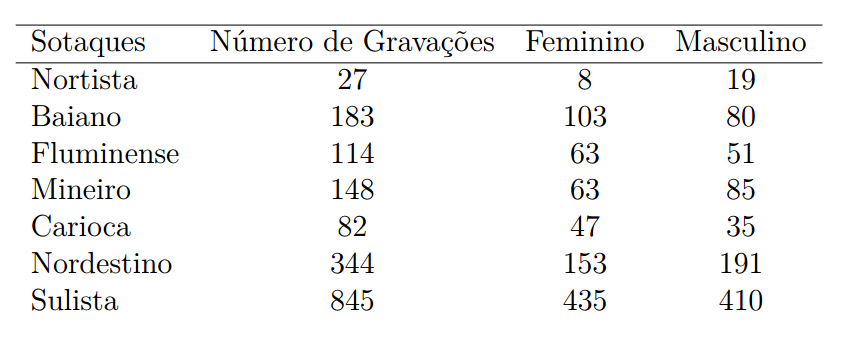
\includegraphics[width=0.6\textwidth]{images/tabBraccent.png}
\fonte{retirado de \citeonline{batista2019estudo}}
\end{table}



\section{MÉTRICAS DE COMPARAÇÃO}

Neste trabalho foi utilizado a métrica de Levenshtein Distance para analisar o desempenho das API's. A distância de Levenshtein foi introduzida em 1995 por Kessler para medir a distância entre dialetos \cite{kessler1995computational}. Dada pelo número mínimo de operações necessárias para transformar um trecho no outro. Existindo três tipos de operações para realizar o processamento: inserção, exclusão e substituição de caracteres \cite{beijering2008predicting}.

Seu funcionamento ocorre pelo preenchimento de uma matriz (n) x (m), na qual n e m são o número de caracteres das duas \textit{strings} a serem comparadas. Como exemplo, vamos comparar as \textit{strings} ``TESTE'' em ``TECLA'', que origina uma matriz 5 x 5, conforme \autoref{LevenshteinPasso1}. 

\begin{quadro}[h]
\caption{Passo inicial da execução da métrica de Levenshtein}
\label{LevenshteinPasso1}
\centering
\begin{tabular}{cc|c|c|c|c|c|}
\textbf{}  & \textbf{} & \textbf{T} & \textbf{E} & \textbf{S} & \textbf{T} & \textbf{E} \\ 
\textbf{}  & 0         & 1          & 2          & 3          & 4          & 5          \\ \hline
\textbf{T} & 1         &            &            &            &            &            \\ \hline
\textbf{E} & 2         &            &            &            &            &            \\ \hline
\textbf{C} & 3         &            &            &            &            &            \\ \hline
\textbf{L} & 4         &            &            &            &            &            \\ \hline
\textbf{A} & 5         &            &            &            &            &            \\ \hline
\end{tabular}
\fonte{elaborado pelo próprio autor (2021)}
\end{quadro}

\begin{quadro}[h!]
\caption{Passo intermediário da execução da métrica de Levenshtein}
\label{LevenshteinPasso2}
\centering
\begin{tabular}{cc|c|c|c|c|c|}
\textbf{}  & \textbf{} & \textbf{T} & \textbf{E} & \textbf{S} & \textbf{T} & \textbf{E} \\ 
\textbf{}  & 0         & 1          & 2          & 3          & 4          & 5          \\ \hline
\textbf{T} & 1         & 0          & 1          &           &           &           \\ \hline
\textbf{E} & 2         &     1       &      0      &            &            &            \\ \hline
\textbf{C} & 3         &            &            &            &            &            \\ \hline
\textbf{L} & 4         &            &            &            &            &            \\ \hline
\textbf{A} & 5         &            &            &            &            &            \\ \hline
\end{tabular}
\fonte{elaborado pelo próprio autor (2021)}
\end{quadro}
\begin{quadro}[h]
\caption{Passo final da execução da métrica de Levenshtein}
\label{LevenshteinPasso3}
\centering
\begin{tabular}{cc|c|c|c|c|c|}
\textbf{}  & \textbf{} & \textbf{T} & \textbf{E} & \textbf{S} & \textbf{T} & \textbf{E} \\ 
\textbf{}  & 0         & 1          & 2          & 3          & 4          & 5          \\ \hline
\textbf{T} & 1         & 0          & 1          & 2          & 3          & 4          \\ \hline
\textbf{E} & 2         & 1          & 0          & 1          & 2          & 3          \\ \hline
\textbf{C} & 3         & 2          & 1          & 1          & 2          & 3          \\ \hline
\textbf{L} & 4         & 3          & 2          & 2          & 2          & 3          \\ \hline
\textbf{A} & 5         & 4          & 3          & 3          & 3          & 3          \\ \hline
\end{tabular}
\fonte{elaborado pelo próprio autor (2021)}
\end{quadro}
%, pois em todas comparações pelo menos uma das \textit{strings} é vazia. Portanto a única operação que é realizada é de inclusão de caractere até formar a outra \textit{string}. A posição (1,1) começa com 0 (zero). 
Dando início ao preenchimento das células restantes, existem duas possibilidades que devem ser observadas para realizar o preenchimento. Devemos verificar se as  \textit{substring} são iguais ou não. Analisando a célula (1,1), deve-se comparar os caracteres 'T' e 'T', nesse caso o campo é preenchido com o valor 0 (zero), pois são iguais. Como os caracteres adicionados em cada \textit{substring} são os mesmos, a matriz é transposta. %não é necessário realizar nenhuma operação extra, portanto seu valor é igual a diagonal superior esquerda, que representa o resultado das mesmas Strings desconsiderando ambos caracteres.

Avançando um caractere, compara-se as \textit{substrings} ``T'' com ``TE'' para a posição (1,2), a comparação de ``TE'' com ``T'' para a posição (2,1) e comparação de ``TE'' com ``TE'' para a posição (2,2). Cada célula é preenchida da seguinte forma: à esquerda (custo da inclusão), acima (custo da exclusão) e na diagonal (custo da substituição). O custo de inclusão é 1, o custo de exclusão é 1 e o custo de substituição é 0 (são iguais).

%da célula atual e então é somado um ao valor encontrado. Na posição (1,2) da matriz, os últimos caracteres da \textit{substring} são diferentes ('T' e 'E'), portanto Portanto a terceira célula da segunda linha deve ser preenchido com o valor 1.


Continua-se o preenchimento dos campos restantes seguindo o processo explicado anteriormente. Na próxima comparação, \textit{substrings} ``TEC'' e ``TES'', na diagonal (3,3) o valor é 1, pois deve-se substituir um caractere. E os custos de inclusão (células na linha até a diagonal ou células à esquerda) e exclusão (células na coluna até a diagonal ou células acima) são preenchidos. Ao final, a matriz fica como mostrado no  \autoref{LevenshteinPasso3}. 

Cada célula da matriz representa o custo mínimo para transformar a respectiva parte da \textit{string} na outra, portanto, a última célula da matriz representa o valor mínimo para transformar a \textit{string} ``TESTE'' em ``TECLA''. A posição (5,5) é o resultado da distância de  Levenshtein, que é o custo mínimo para transformar ``TESTE'' em ``TECLA'', que são 3 operações, de acordo com o algoritmo.



Além do Levenshtein, foi utilizado Levenshtein Normalizado, que é obtido através da divisão do valor da distância Levenshtein pelo tamanho da maior \textit{string}, resultando em um valor percentual da proximidade entre as duas \textit{strings}. Utilizando o exemplo anterior, o Levenshtein Normalizado teria como resultado 0,6 (3 dividido por 5), logo, 60\% de semelhança entre as duas \textit{strings}.




% ---
% ------------------------ Desenvolvimento ------------------------
% ---
\chapter[DESENVOLVIMENTO]{DESENVOLVIMENTO}


%\section{Speech Recognition}
Neste trabalho foi feita a comparação entre duas APIs que realizam a transcrição de áudio para texto, sendo uma delas do Google, conhecida como Cloud Speech-to-Text e a Wit.ai que é utilizada pelo Facebook em bots de chat do messenger. Estas ferramentas processam arquivos de áudio afim de transcrever a fala para texto. Foi utilizado a linguagem Python e a biblioteca Speech Recognition criada por \citeonline{SpeechRecognition} que serve para simplificar a interação do código desenvolvido com a API. Neste capítulo será detalhado como foi implementado o ambiente para análise do desempenho das APIs.

\begin{figure}[h!]
\centering
\caption{Diagrama das APIs selecionadas para análise}
\label{diagramaAPI}
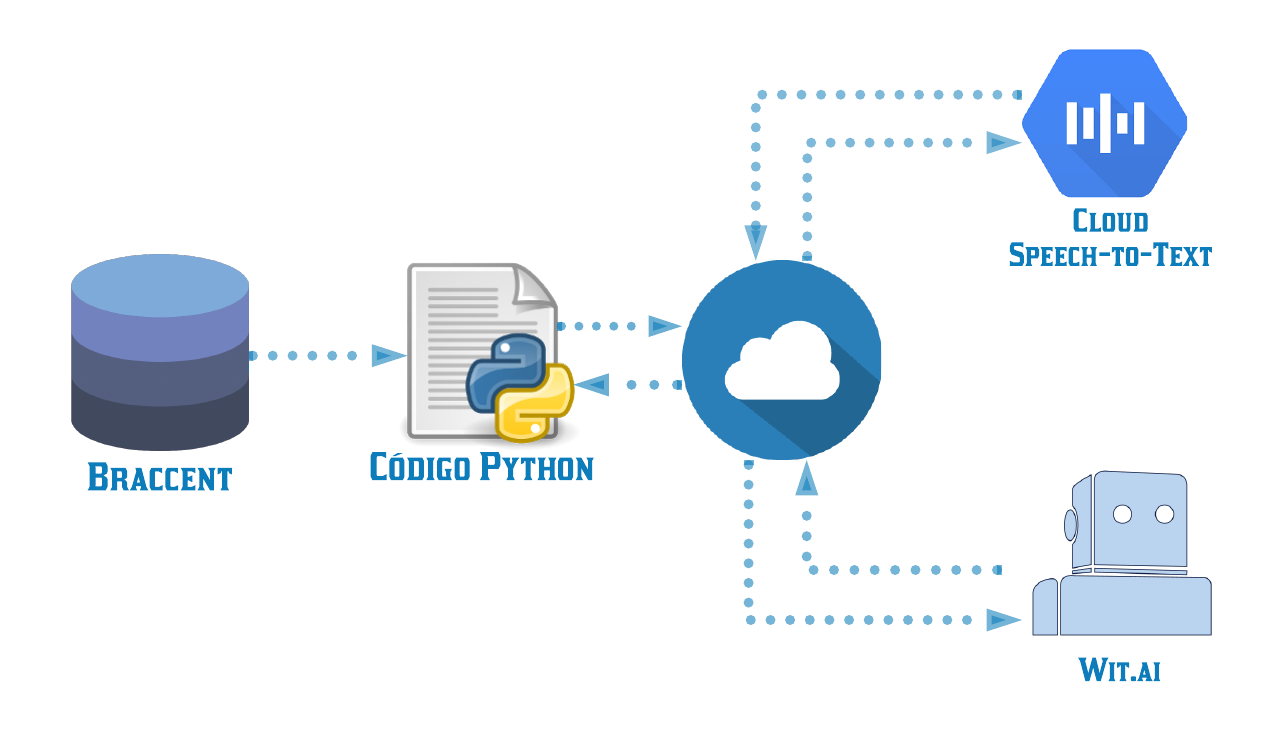
\includegraphics[width=115mm]{images/Diagramas/APIs.png}
\fonte{Elaborado pelo próprio autor (2021).}
\end{figure}

Conforme ilustrado na Figura \ref{diagramaAPI}, o funcionamento do código ocorre de acordo com o seguinte fluxo:

\begin{enumerate}[itemsep=2pt,parsep=2pt]
    \item O código desenvolvido em Python coleta o áudio da base de dados Braccent;
    \item O código Python desenvolvido solicita o processamento do áudio através da nuvem para a respectiva API;
    \item O código fica em modo \emph{stand by} enquanto aguarda a resposta;
    \item A API retorna a resposta;
    \item O código apresenta o texto referente a transcrição do áudio para o usuário;
\end{enumerate}

\section{GOOGLE CLOUD SPEECH API}

A API foi escolhida por ser de uma empresa de  reconhecimento mundial e disponibilizar 300 dólares de crédito com validade de um ano, considerado como suficiente para a conclusão do projeto, além de possuir suporte para o idioma português do Brasil (pt-BR), sendo um requisito obrigatório.

Para começar a utilizá-la é necessário fazer o download da biblioteca através do comando 'pip install google-api-python-client' no prompt de comando, e então criar uma conta no \emph{Google Cloud Platform}, através do link \footnote{https://cloud.google.com/speech-to-text}, clicando no botão 'Comece a usar gratuitamente' no canto superior direito como é possível observar na Figura \ref{Cloudexplicação}, que vai redirecionar para uma tela em que deve acessar uma conta do Google e então preencher um formulário de cadastro composto por duas etapas. 


\begin{figure}[h!]
\centering
\caption{Tela explicativa da Cloud Speech-to-Text}
\label{Cloudexplicação}
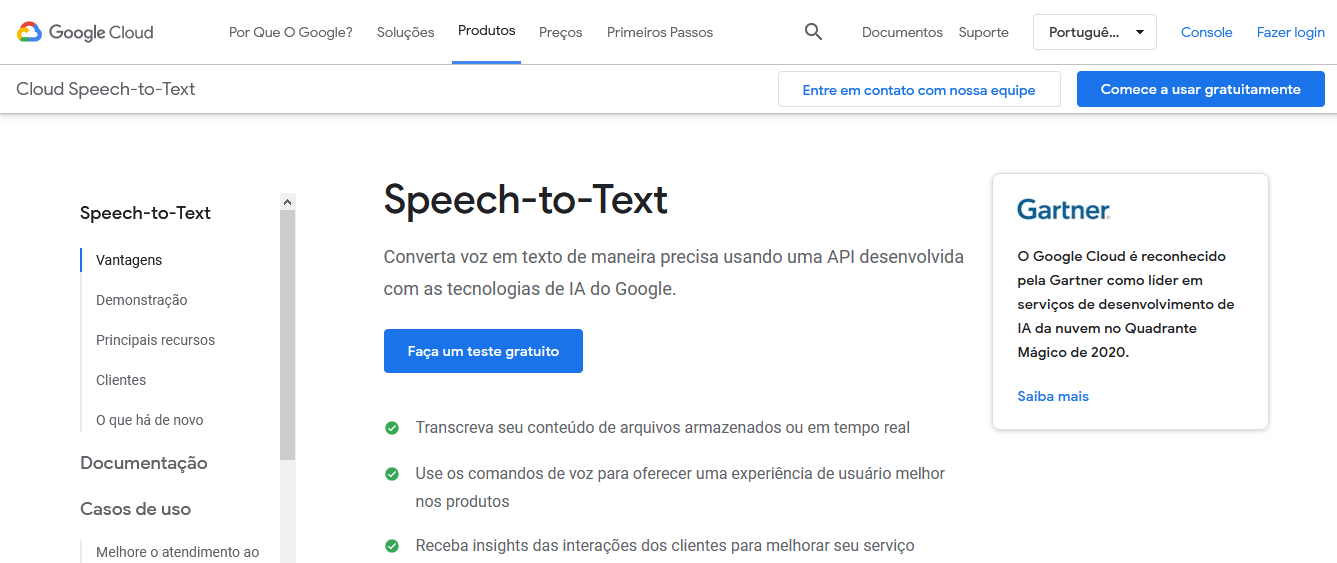
\includegraphics[width=140mm]{images/ConfigurarGoogle/Google_TelaInicial.PNG}
\fonte{Elaborado pelo próprio autor (2021).}
\end{figure}


Na etapa 1 deve ser informado (Figura \ref{CloudCadastro1}) o país de onde vai acessar e ler e concordar com os termos ``Custom Search API Termos de Serviço'' e ``Termos de Serviço do período de teste gratuito do Google Cloud Platform''. Feito isso e pressionando o botão continuar, são solicitados seus dados de endereço (Figura \ref{CloudCadastro2a} e forma de pagamento Figura \ref{CloudCadastro2b}).

\begin{figure}[h!]
\centering
\caption{Tela de Cadastro da Cloud Speech-to-Text, etapa 1}
\label{CloudCadastro1}
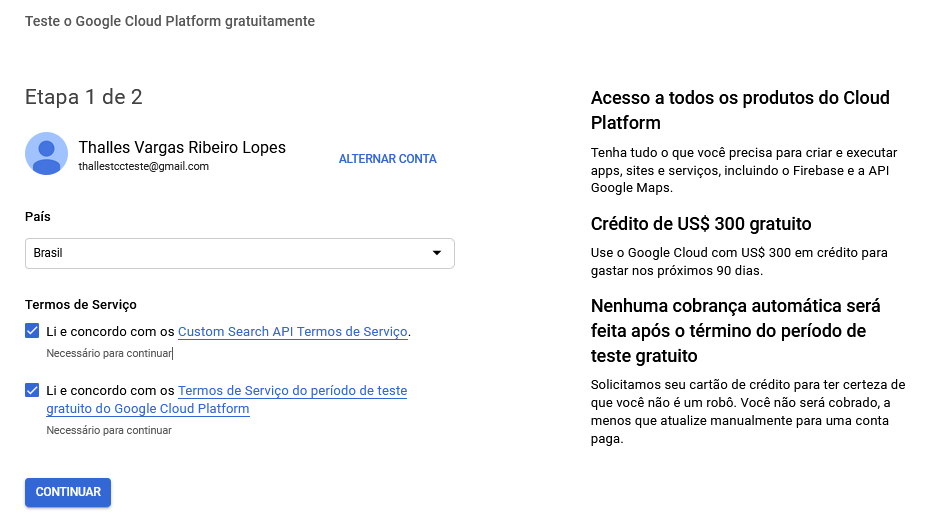
\includegraphics[width=140mm]{images/ConfigurarGoogle/cadastroetapa01.PNG}
\fonte{tela do Google Cloud (2021).}
\end{figure}

\begin{figure}[h!]
\centering
\caption{Tela de Cadastro da Cloud Speech-to-Text, etapa 2A}
\label{CloudCadastro2a}
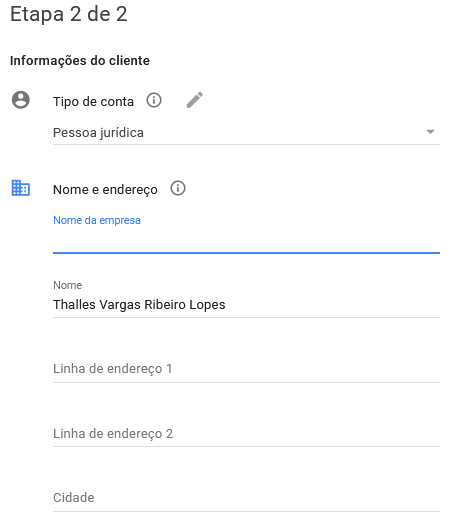
\includegraphics[width=80mm]{images/ConfigurarGoogle/cadastroetapa02a.PNG}
\fonte{tela do Google Cloud (2021).}
\end{figure}

\begin{figure}[h!]
\centering
\caption{Tela de Cadastro da Cloud Speech-to-Text, etapa 2B}
\label{CloudCadastro2b}
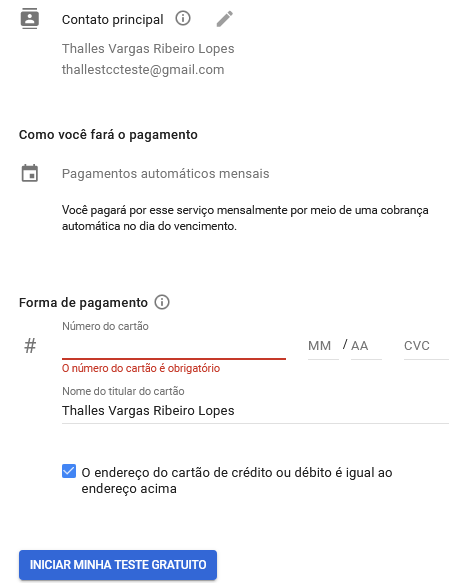
\includegraphics[width=80mm]{images/ConfigurarGoogle/cadastroetapa02b.PNG}
\fonte{tela do Google Cloud (2021).}
\end{figure}
\FloatBarrier


Com a conta criada e com acesso a plataforma do Google, basta realizar a busca no campo que se encontra na parte de cima da tela (Figura \ref{plataformaGoogle}) digitando 'Speech-to-Text e ativar a ferramenta em seu perfil pressionando o comando 'Ativar' (Figura \ref{AtivarAPI}), feito isso, terá acesso ao ambiente de configuração da sua API (Figura \ref{telainicialAPI}) onde deve acessar o menu 'Credenciais' e preencher os campos necessários (Figuras \ref{criarCredencial} e \ref{criarCredencial2}) para receber a credencial que vai ser utilizada na chamada da API (Figura \ref{chaveCriada}).

\begin{figure}[h!]
\centering
\caption{Tela Inicial da Plataforma Google}
\label{plataformaGoogle}
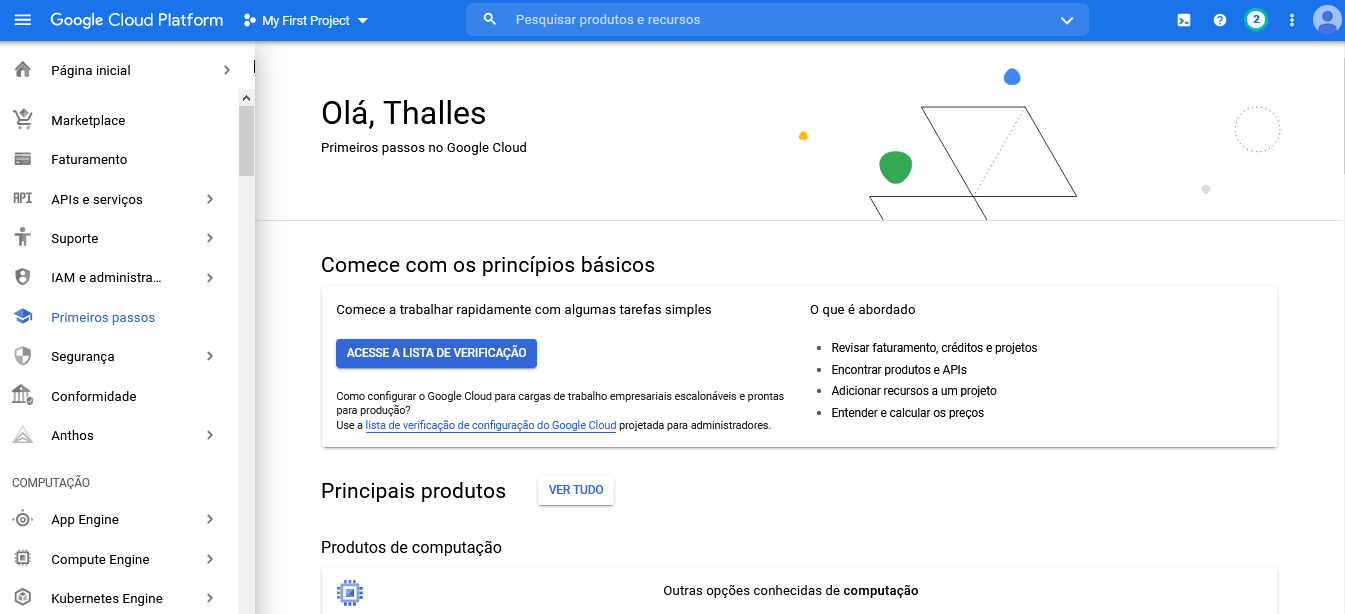
\includegraphics[width=150mm]{images/ConfigurarGoogle/telainicial.PNG}
\fonte{tela do Google Cloud (2021).}
\end{figure}

\begin{figure}[h!]
\centering
\caption{Tela para Ativar a API Speech-To-Text na conta}
\label{AtivarAPI}
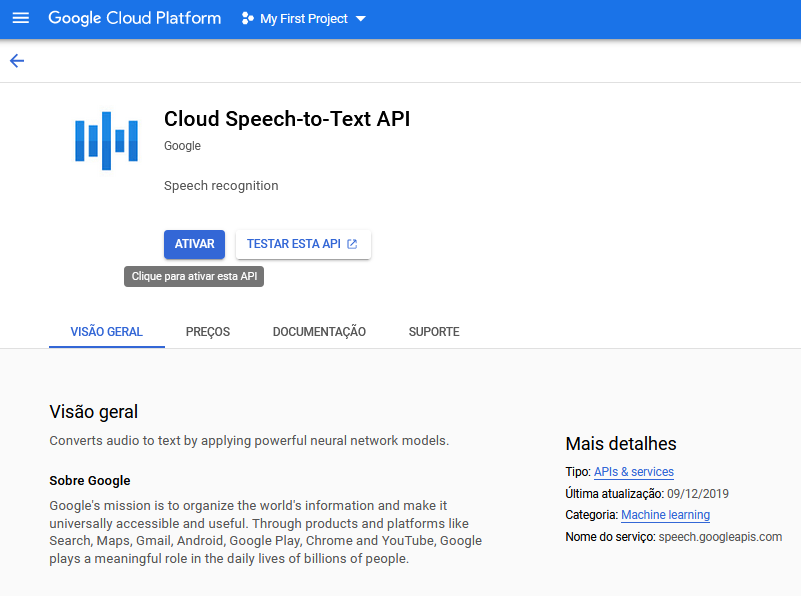
\includegraphics[width=150mm]{images/ConfigurarGoogle/AtivarAPI.PNG}
\fonte{tela do Google Cloud (2021).}
\end{figure}

\begin{figure}[h!]
\centering
\caption{Tela inicial da API Speech-To-Text}
\label{telainicialAPI}
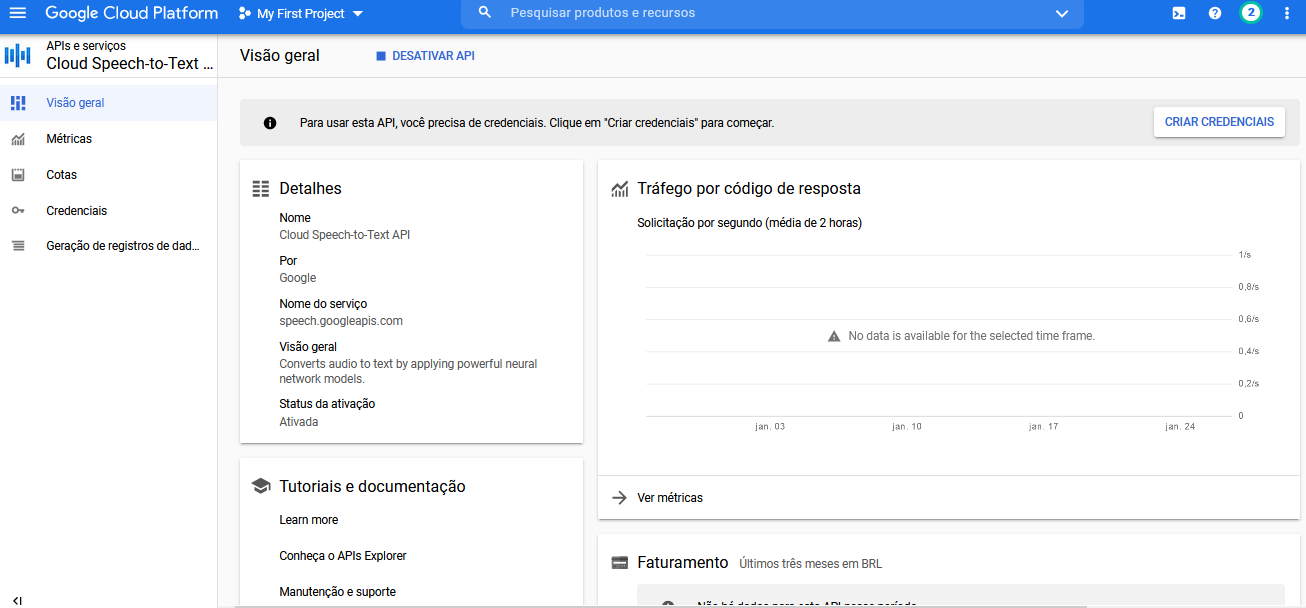
\includegraphics[width=150mm]{images/ConfigurarGoogle/telainicialSpeechToText.PNG}
\fonte{tela do Google Cloud (2021).}
\end{figure}

\begin{figure}[h!]
\centering
\caption{Tela de cadastro de Credencial da API Speech-To-Text, etapa 01}
\label{criarCredencial}
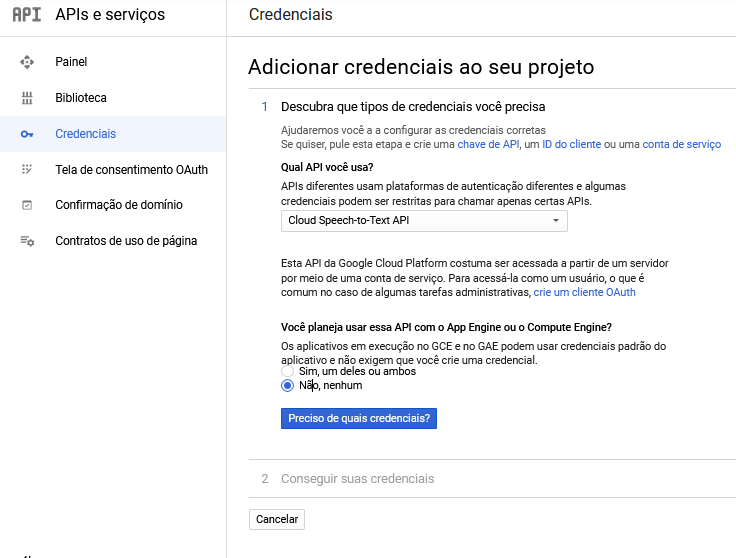
\includegraphics[width=150mm]{images/ConfigurarGoogle/criarCredencialEtapa1.PNG}
\fonte{tela do Google Cloud (2021).}
\end{figure}

\begin{figure}[h!]
\centering
\caption{Tela de cadastro de Credencial da API Speech-To-Text, etapa 02}
\label{criarCredencial2}
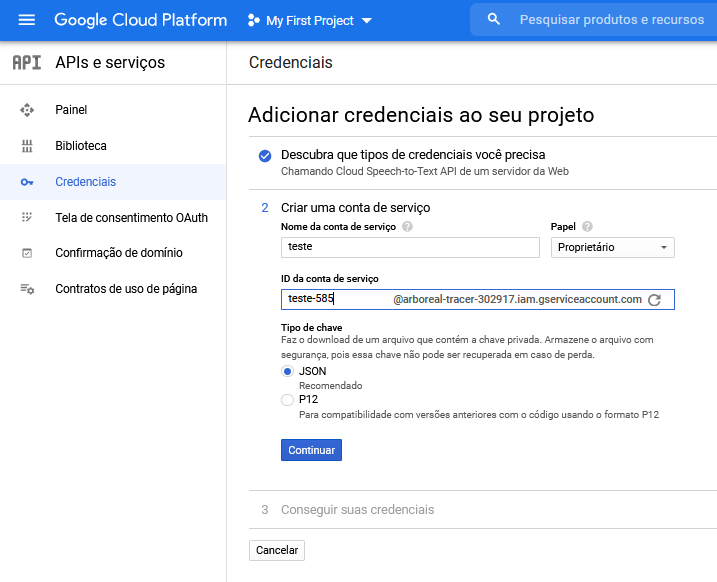
\includegraphics[width=150mm]{images/ConfigurarGoogle/criarCredencialEtapa2.PNG}
\fonte{tela do Google Cloud (2021).}
\end{figure}

\begin{figure}[h!]
\centering
\caption{Tela de sucesso da criação de credencial}
\label{chaveCriada}
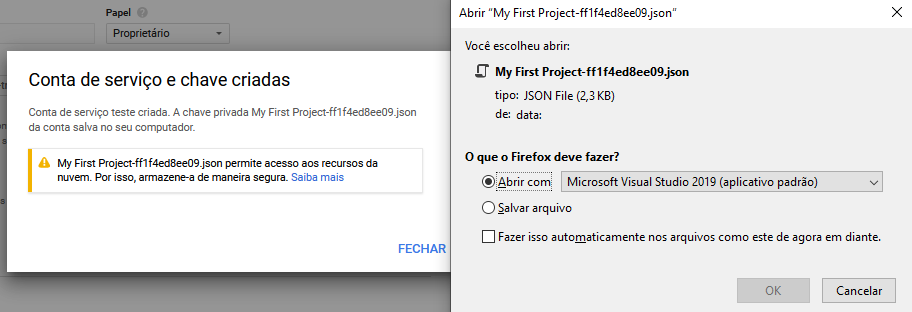
\includegraphics[width=150mm]{images/ConfigurarGoogle/chaveCriada.PNG}
\fonte{tela do Google Cloud (2021).}
\end{figure}

\FloatBarrier

O código descrito no \autoref{googleCloudAPI} demonstra a chamada da API para os testes do projeto. Iniciando importando a biblioteca Speech Recognition que vai realizar o intermédio entre a API e o programa. Na linha 5 é passado o caminho para a pasta que a base dados BRACCENT se encontra. Na linha 6 deve ser atribuído à variável ``GOOGLE\_CLOUD\_SPEECH\_CREDENCIALS'' a credencial gerada na plataforma do Google. Na linha 8 é iniciado um \textit{loop} que deve verificar todos os arquivos que se encontram no diretório passado como parâmetro e então enviar todos que forem arquivos '.wav' para a API do Google realizar a transcrição. Na requisição na linha 17 e 18, passam-se como parâmetros o áudio, a língua que está sendo transcrita e as credenciais, e o processo fica aguardando a resposta da API. Se a chave e o áudio fornecidos forem válidos, é retornado a resposta em formato de \textit{string}. 

\begin{quadro}[h!]
\centering
\caption{Código para realizar a chamada da API \emph{Google Cloud API}}
\label{googleCloudAPI}
\lstdefinestyle{nonumbers}
{numbers=none}
\begin{lstlisting}[language=Python]
import speech_recognition as sr
from os import path
import os

directory = r'C:\TCC\BRAccent001\Stereo\Baiano\Masculino'
GOOGLE_CLOUD_SPEECH_CREDENTIALS = ''KEY''

for filename in os.listdir(directory):
    if filename.endswith('.wav'):
        AUDIO_FILE = path.join(directory, filename)

        r = sr.Recognizer()
        with sr.AudioFile(AUDIO_FILE) as source:
            audio = r.record(source)
            
        try:
            print(r.recognize_google_cloud(audio, language='pt-BR', credentials_json=GOOGLE_CLOUD_SPEECH_CREDENTIALS))
        except sr.UnknownValueError:
            print(''Google Cloud Speech could not understand audio'')
        except sr.RequestError as e:
            print(''Could not request results from Google Cloud Speech service; {0}''.format(e))
\end{lstlisting}
\fonte{Elaborado pelo autor (2021).}
\end{quadro}

Caso finalize a resposta sem nenhum erro, é retornado o texto ou a \textit{string} do áudio. Existem duas exceções definidas para possíveis problemas, o primeiro para o caso da API do Google não conseguir identificar quais palavras estão sendo pronunciadas (linha 18) e o segundo para o erro de conexão com a API (Linha 20). 

\section{WIT.AI}

A {Wit.ai} foi selecionada pela sua  facilidade de uso, ser completamente gratuita e possuir suporte para o idioma português do Brasil (pt-BR). A empresa  somente solicita que seja informada no caso em que há chamadas com muita frequência, por exemplo, uma  chamada por segundo. Neste trabalho não foi necessário o uso intenso da API e portanto não houve essa notificação.

Para começar a utilizá-lo deve acessar o site\footnote{https://wit.ai} e realizar o cadastro através de uma conta do Facebook ou Github, conforme é possível ver na parte inferior direita da Figura \ref{witInicio}. Após ter acessado a conta é apresentada a listagem de suas aplicações (Apps) criadas (Figura \ref{witListagemApps}), no caso de ser a primeira deve ser acessado o botão '\textbf{+ New App}' que vai abrir a tela de cadastro de App (Figura \ref{witCreateApp}) onde é necessário informar o nome da App, a linguagem que vai ser utilizada na transcrição e a privacidade da App. 

\begin{figure}[h!]
\centering
\caption{Tela inicial do site Wit.ai}
\label{witInicio}
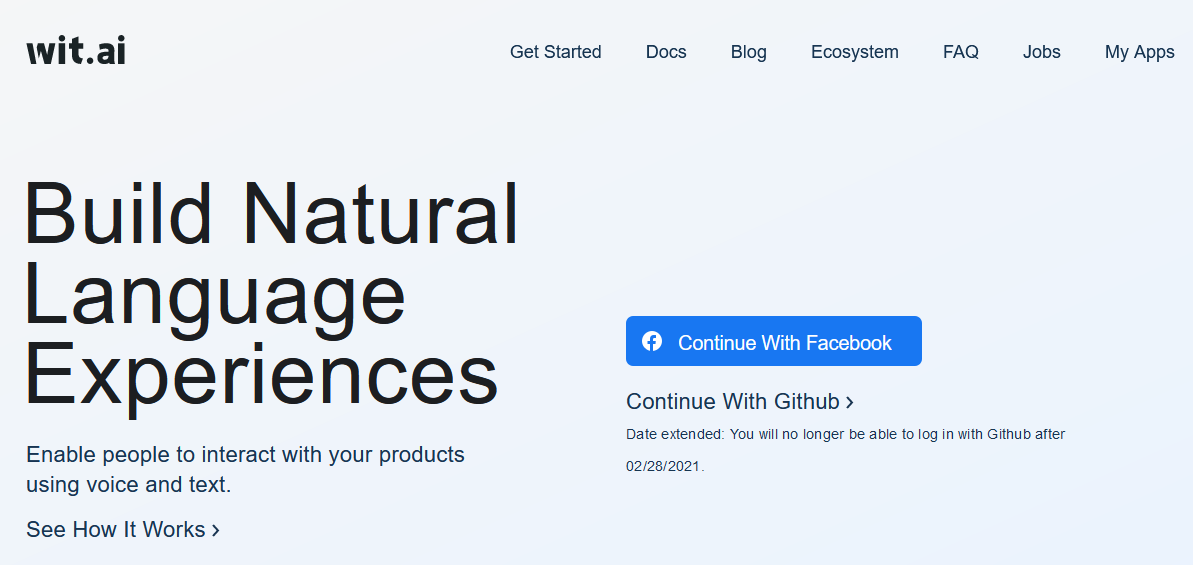
\includegraphics[width=150mm]{images/ConfigurarWit/witTelaInicial.PNG}
\fonte{tela do Wit.ai (2021).}
\end{figure}

\begin{figure}[h!]
\centering
\caption{Tela de listagem das Apps da conta Wit}
\label{witListagemApps}
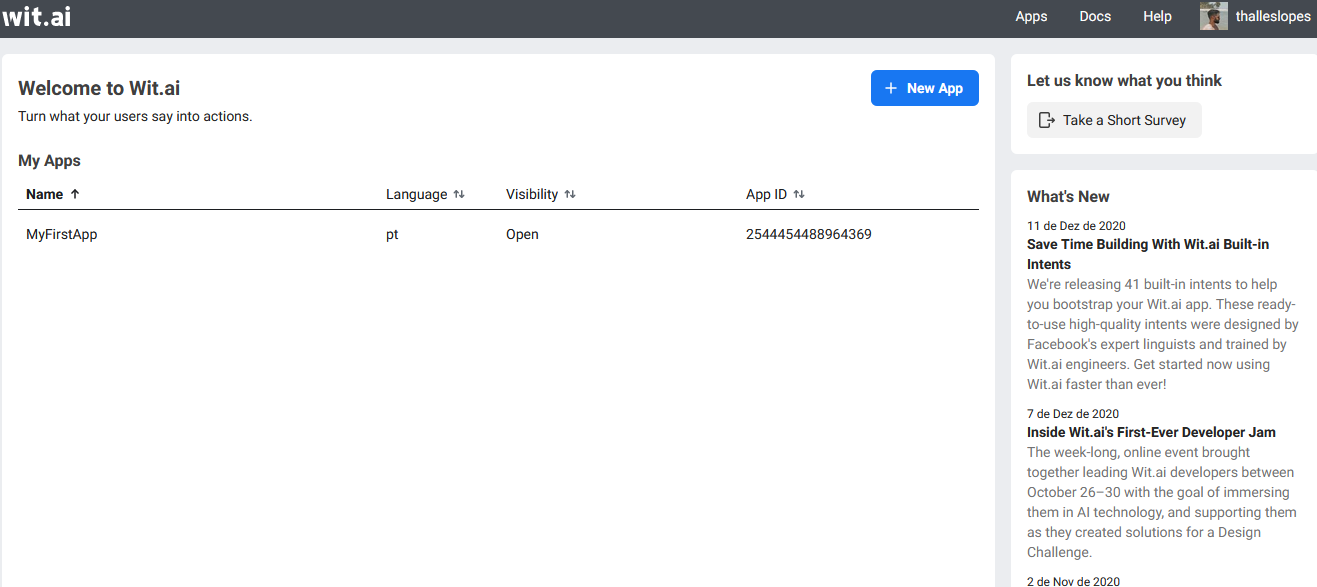
\includegraphics[width=150mm]{images/ConfigurarWit/witListagemApp.PNG}
\fonte{tela do Wit.ai (2021).}
\end{figure}

\begin{figure}[h!]
\centering
\caption{Tela de cadastro de App da Wit}
\label{witCreateApp}
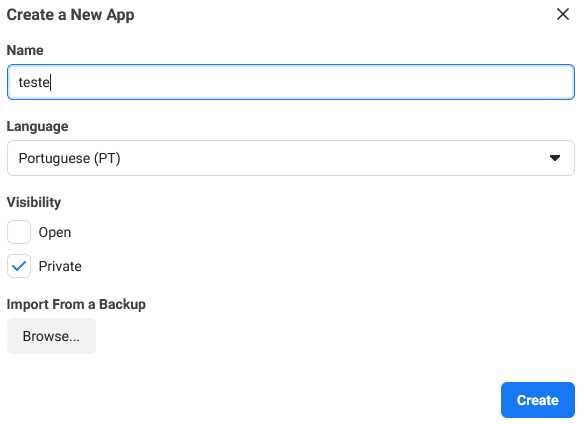
\includegraphics[width=100mm]{images/ConfigurarWit/witCreateApp.PNG}
\fonte{tela do Wit.ai (2021).}
\end{figure}

\FloatBarrier
Clicando no botão \textbf{Create} para confirmar a criação, o usuário é  redirecionado  para a tela inicial da App (Figura \ref{witAppInicio}) que apresenta o histórico de transcrições realizadas, caso tenha acabado de criar a App, nenhum dado vai ser apresentado. Acessando o menu na lateral esquerda, '\textbf{Settings}' dentro de '\textbf{Management}', são apresentadas as configurações da App (Figura \ref{witAppSettings}), onde permite configurar informações referentes a App, como por exemplo o '\textbf{Server Acess Token}' que é necessário para realizar a chamada da API.



\begin{figure}[h!]
\centering
\caption{Tela Inicial da App da Wit.ai}
\label{witAppInicio}
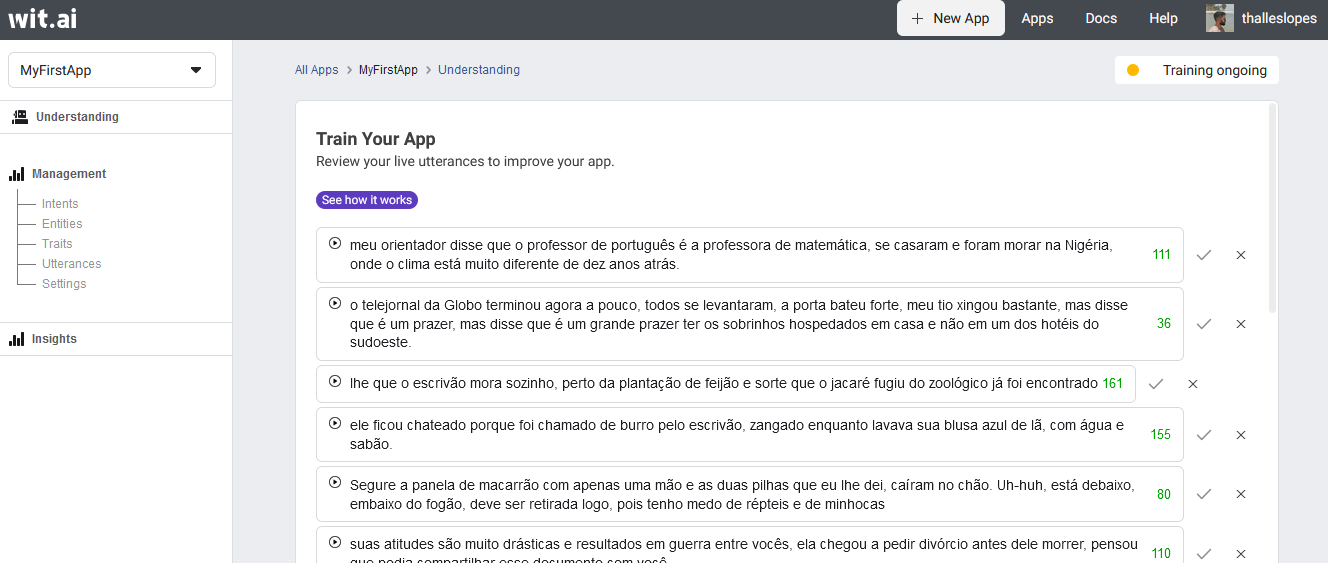
\includegraphics[width=160mm]{images/ConfigurarWit/witHistoricoTranscricao.PNG}
\fonte{tela do Wit.ai (2021).}
\end{figure}

\begin{figure}[h!]
\centering
\caption{Tela de configuração da App da Wit.ai}
\label{witAppSettings}
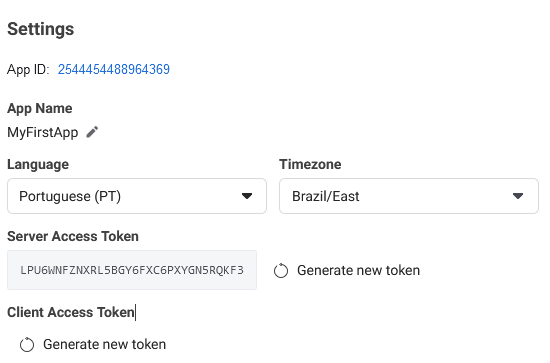
\includegraphics[width=110mm]{images/ConfigurarWit/witSettings.PNG}
\fonte{tela do Wit.ai (2021).}
\end{figure}

\FloatBarrier

Com o \textit{token} gerado já é possível utilizar a biblioteca Speech Recognition para a transcrição com a Wit. No Quadro \autoref{witAPI} apresenta o código de chamada da API, que funciona de maneira similar à do Google Cloud.


\begin{quadro}[h]
\centering
\caption{Código para realizar a chamada da API \emph{Wit.ai}}
\label{witAPI}
\lstdefinestyle{nonumbers}
{numbers=none}
\begin{lstlisting}[language=Python]
import speech_recognition as sr
from os import path
import os
directory = r'C:\TCC\BRAccent001\Mono\Baiano\Feminino'

WIT_AI_KEY = "Wit.ai_key" 

for filename in os.listdir(directory):
    if filename.endswith(".wav"):
        AUDIO_FILE = path.join(directory, filename)

        r = sr.Recognizer()
        with sr.AudioFile(AUDIO_FILE) as source:
            audio = r.record(source) 

        try:	
            print(r.recognize_wit(audio, key=WIT_AI_KEY))
        except sr.UnknownValueError:
            print("Wit.ai could not understand audio")
        except sr.RequestError as e:
            print("Could not request results from Wit.ai service; {0}".format(e))
            
\end{lstlisting}
\fonte{Elaborado pelo autor (2021).}
\end{quadro}

O código inicia importando a biblioteca Speech Recognition que vai realizar o intermédio entre a API e o programa. Na linha 4 é passado o caminho para a pasta que a base dados BRACCENT se encontra. Na linha 6 deve ser atribuído à variável ''WIT\_AI\_KEY'' o \textit{token} gerado na plataforma da Wit. Na linha 8 é iniciado um \textit{loop} que deve verificar todos os arquivos que se encontram no diretório passado como parâmetro e então enviar todos que forem arquivos '.wav' para a API da Wit realizar a transcrição. 

 
Ao realizar a requisição na linha 18, passando como parâmetros o áudio e a chave, o processo fica parado aguardando a resposta da API (o parâmetro de língua é mantido nas configurações da App). Se a chave e o áudio fornecidos forem válidos, é retornada a resposta em formato de \textit{string}.

\section{TRATAMENTO DE PONTUAÇÃO}

Posteriormente ao inicio do trabalho, foi feito o processamento das transcrições para remover as pontuações, afim de produzir duas planilhas distintas para serem analisadas, conforme a necessidade de realizar uma comparação mais equivalente, uma vez que o Google Cloud não realiza a utilização de pontuação.

Como é possível observar no \autoref{removerPontuacao}, nas linhas 1 e 2 são importadas as bibliotecas necessárias para manipular as planilhas. Na linha 4 é selecionado a planilha que possui os dados para serem tratados e na linha 5 a aba da planilha. Na linha 6 são definidos todas as pontuações que devem ser removidas do texto. Na linha 8 é realizado um loop para percorrer todas as células que possuem o texto verificando se algum dos caracteres é trata de uma pontuação, se for o caso ela deve ser removida (substituída por uma String vazia). Após percorrer todos os caracteres do texto o código deve ajustar todas as letras para minúscula, através do comando feito na linha 14.

\begin{quadro}[h]
\centering
\caption{Código para remover a pontuação \emph{Wit.ai}}
\label{removerPontuacao}
\lstdefinestyle{nonumbers}
{numbers=none}
\begin{lstlisting}[language=Python]
import openpyxl
from openpyxl import load_workbook

wb = load_workbook(filename = ''2 Google Cloud - BRACCENT.xlsx'')
ws = wb['Sulista']
pontuacao = '''!()-[]{};:'"\,<>./?@#$%^&*_~'''

for row in ws.iter_rows(min_row=2, max_col=4, max_row=1000, values_only=True):
    frase = row[2]
    for ele in frase:  
        if ele in pontuacao:  
            frase = frase.replace(ele, '')  
    
    frase = frase.lower()
    print(frase)
\end{lstlisting}
\fonte{Elaborado pelo autor (2021).}
\end{quadro}



\section{COLETA DAS MÉTRICAS DE COMPARAÇÃO}

Para a coleta das métricas de comparação de texto, existem dois resultados diferenciados: considerando a pontuação e sem considerar a pontuação. A pontuação das frases são as vírgulas, pontos finais, aspas e parágrafos (letra maiúscula). O resultado da ferramenta Google Cloud não utiliza quaisquer tipos de pontuação, diferente da ferramenta Wit.ai em que sua transcrição contém vírgulas, pontos finais e letras maiúsculas de início de parágrafo. O Wit.ai só não avalia as aspas. 

%\todo[inline]{como referenciar links?}
Para calcular a similaridade das transcrições feitas pelas API's com as respectivas frases originais, foi utilizada a biblioteca 'python-string-similarity'\footnote{\url{ https://github.com/luozhouyang/python-string-similarity\#python-string-similarity}} que fornece diversas funções para comparar duas \textit{strings}. Para começar a utilizar a biblioteca é necessário fazer o \textit{download}  através do \textbf{cmd} com o comando \textbf{pip install -U strsimpy}. Terminando a instalação, o Python já está configurado para a utilização das funções da biblioteca.


\begin{quadro}[h]
\centering
\caption{Código para calcular a similaridade \emph{Wit.ai}}
\label{métricaLev}
\lstdefinestyle{nonumbers}
{numbers=none}
\begin{lstlisting}[language=Python]
import openpyxl
from openpyxl import load_workbook
from strsimpy.jaro_winkler import Levenshtein

wb = load_workbook(filename = ''Google Cloud - BRACCENT.xlsx'')
ws = wb[''Sulista'']

levenshtein = Levenshtein()
for row in ws.iter_rows(min_row=1, max_col=3, max_row=1000, values_only=True):
    print(levenshtein.distance(row[1], row[2]))
\end{lstlisting}
\fonte{Elaborado pelo autor (2021).}
\end{quadro}


O código utilizado para comparar o resultado das API's é apresentado no \autoref{métricaLev}. Nas Linhas 1, 2 apenas são realizadas importações necessárias para leitura do arquivo XLS e na Linha 3 é feita a importação da métrica Levenshtein da biblioteca \textbf{strsimpy}. Na Linha 5 é selecionado o arquivo para ser lido e na Linha 6 a aba da planilha. A Linha 10 é  um \textit{loop} que vai rodar da primeira linha (\textbf{min\_row=1}) e terceira coluna (\textbf{max\_col=3}) até a linha mil (\textbf{max\_row=1000}) imprimindo o resultado do cálculo de similaridade entre a coluna referente a frase original (\textbf{row[1]}) e a transcrição da API (\textbf{row[2]}).

Há variações deste código na Linha 5, em que o nome do arquivo é alterado para o resultado do Google Cloud sem pontuação, e para o Wit.ai, com e sem pontuação. As abas também são alteradas na Linha 6. E para se fazer o cálculo do Levenshtein normalizado, a Linha 3 e Linha 8 são alteradas como mostrado no Quadro \ref{métricaNormalizedLev}.


\begin{quadro}[h]
\centering
\caption{Código para calcular a similaridade \emph{Wit.ai}}
\label{métricaNormalizedLev}
\lstdefinestyle{nonumbers}
{numbers=none}
\begin{lstlisting}[language=Python]
import openpyxl
from openpyxl import load_workbook
from strsimpy.normalized_levenshtein import NormalizedLevenshtein

wb = load_workbook(filename = ''2 Wit - BRACCENT.xlsx'')
ws = wb[''Sulista'']

normalized_levenshtein = NormalizedLevenshtein()
for row in ws.iter_rows(min_row=2, max_col=4, max_row=1000, values_only=True):
    print(normalized_levenshtein.similarity(row[1], row[2]))
\end{lstlisting}
\fonte{Elaborado pelo autor (2021).}
\end{quadro}



\vspace*{\fill}

{~~~~~~~~~}


{~~~~~~~~~}




% ---
% ------------------------ Resultados ------------------------
% ---
\chapter[EXPERIMENTOS, RESULTADOS E DISCUSSÃO]{EXPERIMENTOS, RESULTADOS E DISCUSSÃO}

Neste capítulo serão apresentados e discutidos os resultados obtidos através do processamento dos áudios descritos no capítulo anterior. O principal objetivo é mapear como foi o acerto das ferramentas de transcrição usadas nos experimentos: Google Speech API e Wit.ai. Primeiro serão apresentadas as métricas de forma geral, depois por sotaque regional, por gênero e por grau de escolaridade.

\section{TRATAMENTO DA BASE DE DADOS BRACCENT}

É importante compreender que o trabalho da  \citeonline{batista2019estudo} teve como objetivo a identificação do sotaque regional e que este trabalho versa sobre a transcrição da fala. Assim, no trabalho de origem, não houve a verificação se cada palavra da frase era pronunciado corretamente pelo voluntário. Para este trabalho, foi feita a seguinte verificação, para cada áudio foram ouvidos pelos menos as duas primeiras palavras. Com isso, alguns áudios foram descartados, pois a pessoa não estava falando a frase identificada e haviam repetições de frases pela mesma pessoa, o  \autoref{Tabela_resumo_sotaque} tem a quantidade de áudio por sotaque e por sexo que foi usada. 


% Please add the following required packages to your document preamble:
% \usepackage{multirow}
\begin{quadro}[h]
\caption{Base de dados selecionada para os experimentos por sotaque e por sexo, totalizando 1.648 áudios, 854 femininos e 794 masculinos.} \label{Tabela_resumo_sotaque}
\centering
\begin{tabular}{|c|c|c|c|}
\hline
\textbf{Sotaque}            & \textbf{Sexo} & \textbf{Quantidade de áudio} & \textbf{Total}       \\ \hline
\multirow{2}{*}{Baiano}   & Feminino      & 99                            & \multirow{2}{*}{173}  \\ \cline{2-3}
                            & Masculino     & 74                           &                     \\ \hline
\multirow{2}{*}{Carioca}     & Feminino      & 47                          & \multirow{2}{*}{81} \\ \cline{2-3}
                            & Masculino     & 34                           &                      \\ \hline
\multirow{2}{*}{Fluminense}    & Feminino      & 61                           & \multirow{2}{*}{110} \\ \cline{2-3}
                            & Masculino     & 49                           &                      \\ \hline
\multirow{2}{*}{Mineiro}    & Feminino      & 58                           & \multirow{2}{*}{137}  \\ \cline{2-3}
                            & Masculino     & 79                           &                      \\ \hline
\multirow{2}{*}{Nordestino} & Feminino      & 158                           & \multirow{2}{*}{333} \\ \cline{2-3}
                            & Masculino     & 175                           &                      \\ \hline
\multirow{2}{*}{Nortista} & Feminino      & 6                          & \multirow{2}{*}{24} \\ \cline{2-3}
                            & Masculino     & 18                          &                      \\ \hline
\multirow{2}{*}{Sulista}    & Feminino      & 425                          & \multirow{2}{*}{790} \\ \cline{2-3}
                            & Masculino     & 365                          &                      \\ \hline
\end{tabular}
\fonte{elaborado pelo próprio autor (2021) com os dados do Braccent.}
\end{quadro}


O trabalho original usava 1.743 amostras de fala, enquanto este trabalho usa 1.648 áudios, sendo 95 áudios a menos. Em comparação com as informações do trabalho original, há 10 áudios a menos no Baiano (4 a menos no feminino e 6 a menos no masculino); 1 a menos no Carioca para o gênero masculino; 4 a menos no fluminense (2 a menos em cada gênero); 11 áudios a menos no sotaque mineiro (5 a menos no feminino e 6 a menos no masculino); 11 a menos no Nordestino (sendo 16 a menos no masculino, mas 5 a mais no feminino); 3 a menos no Nortista (2 a menos no feminino e 1 a menos no masculino) e; 55 a menos no sulista (10 a menos no feminino e 45 a menos no masculino). Os áudios foram conferidos e não se encontrou explicação do porque terem mais áudios do sotaque nordestino feminino na base utilizada. 


\begin{quadro}[h!]
\caption{Base de dados selecionada para os experimentos filtrada por grau de ensino, totalizando 1.648 áudios}
\label{Tabela_resumo_grauDeEnsino}
\centering
\begin{tabular}{|l|c|}
\hline
\textbf{Grau de Ensino} & \multicolumn{1}{l|}{\textbf{Quantidade de áudio}} \\ \hline
Médio Incompleto        & 36                                                \\ \hline
Médio Completo          & 109                                               \\ \hline
Superior Incompleto     & 391                                               \\ \hline
Superior Completo       & 712                                               \\ \hline
Mestrado                & 243                                               \\ \hline
Doutorado               & 157                                               \\ \hline
\end{tabular}
\fonte{elaborado pelo próprio autor (2021) com os dados do Braccent.}
\end{quadro}



O \autoref{Tabela_resumo_grauDeEnsino} apresenta a quantidade de áudios por grau de ensino e por sotaque. Mais detalhes encontram-se no Apêndice A, com dados de grau de escolaridade e município/UF de cidade e estado onde o voluntário reside ou de onde o voluntário considera ser o seu sotaque. Logo, a informação de cidade não é muito confiável, dado que o preenchimento foi feito pelo próprio voluntário e a cidade onde reside não define o seu sotaque, e ainda o voluntário pode considerar que tem um determinado sotaque, mas pode estar enganado. O trabalho original contou com a participação de alunos do curso de Letras da Unicamp para fazer a classificação manual.


Nas próximas seções apresentam os resultados e discussão de forma geral, posteriormente separados por sotaque regional, por gênero e por grau de escolaridade. Em cada seção são apresentados os resultados considerando a pontuação das frases: vírgulas, pontos finais, aspas e parágrafos; e sem considerar a pontuação. 

\section{RESULTADO GERAL}

Nesta seção, consideramos os resultados de toda a base de dados testada. O \autoref{Tabela_geral_com_pontuacao} apresenta os resultados do Google Cloud e do Wit.ai considerando a pontuação e o  \autoref{Tabela_geral_sem_pontuacao} sem a pontuação, os melhores resultados estão em negrito para facilitar a comparação, sendo contabilizado um acerto cada transcrição que fosse igual a frase original.

%COM PONTUAÇÃO
\begin{quadro}[h]
\caption{Resultado das APIs considerando a pontuação} \label{Tabela_geral_com_pontuacao}
\centering
\begin{tabular}{c|c|r|r|l}
\cline{1-4}
\multicolumn{1}{|c|}{Métrica}                                 & Estatística  & \multicolumn{1}{c|}{Google Cloud} & \multicolumn{1}{c|}{Wit.ai} &  \\ \cline{1-4}
\multicolumn{1}{|c|}{\multirow{2}{*}{Levenshtein}}            & Média        & 18,29                           & \textbf{5,85}                      &  \\ \cline{2-4}
\multicolumn{1}{|c|}{}                                        & Mediana      & 14                                & \textbf{4}                           &  \\ \cline{1-4}
\multicolumn{1}{|c|}{\multirow{2}{*}{Normalized Levenshtein}} & Média        & 89\%                            & \textbf{96\%}                      &  \\ \cline{2-4}
\multicolumn{1}{|c|}{}                                        & Mediana      & 91\%                            & \textbf{97\%}                  &  \\ \cline{1-4}
\multicolumn{1}{l|}{}                                         & \# Acertos   & 0                                 & \textbf{81}                          &  \\ \cline{2-4}
\multicolumn{1}{l|}{}                                         & \% de Acerto & 0                                 & \textbf{4,91\%}               &  \\ \cline{2-4}
\end{tabular}
\fonte{elaborado pelo próprio autor (2021)}
\end{quadro}


%SEM PONTUAÇÃO
\begin{quadro}[h]
\caption{Resultado das APIs sem considerar a pontuação} \label{Tabela_geral_sem_pontuacao}
\centering
\begin{tabular}{c|c|r|r|l}
\cline{1-4}
\multicolumn{1}{|c|}{Métrica}                                 & Estatística  & \multicolumn{1}{c|}{Google Cloud} & \multicolumn{1}{c|}{Wit.ai} &  \\ \cline{1-4}
\multicolumn{1}{|c|}{\multirow{2}{*}{Levenshtein}}            & Média        & 13,54                           & \textbf{3,21}                      &  \\ \cline{2-4}
\multicolumn{1}{|c|}{}                                        & Mediana      & 9                                 & \textbf{2}                           &  \\ \cline{1-4}
\multicolumn{1}{|c|}{\multirow{2}{*}{Normalized Levenshtein}} & Média        & 92\%                            & \textbf{98\%}                      &  \\ \cline{2-4}
\multicolumn{1}{|c|}{}                                        & Mediana      & 94\%                            & \textbf{98\%}                      &  \\ \cline{1-4}
\multicolumn{1}{l|}{}                                         & \# Acertos   & 126                               & \textbf{543}                         &  \\ \cline{2-4}
\multicolumn{1}{l|}{}                                         & \% de Acerto & 7,64\%                            & \textbf{32,94\%}             &  \\ \cline{2-4}
\end{tabular}
\fonte{elaborado pelo próprio autor (2021)}
\end{quadro}

Acertar a pontuação é um desafio, logo os resultados considerando a pontuação são piores que sem considerá-la. Mesmo assim, o Wit.ai acertou 81 áudios completos com pontuação. O Google Cloud não retorna resultado com pontuação, logo, a indicação de 0 (zero) acertos.  Ressalta-se que sem considerar a pontuação, essa quantidade aumenta em 6,7 vezes, acertando 543 áudios. Em ambos os quadros, é possível verificar que o Wit.ai teve resultados melhores, em todas as estatísticas, que o Google Cloud. 

\FloatBarrier

\section{RESULTADO POR SOTAQUE REGIONAL}

Nesta seção serão discutidos os resultados por sotaque. O \autoref{Tabela_sotaque_Google_com_pontuacao} apresenta os resultados do Google Cloud considerando a pontuação para os diferentes sotaques e o \autoref{Tabela_sotaque_Google_sem_pontuacao} são os resultados sem considerar a pontuação. Para esta ferramenta, é interessante observar que obteve melhores resultados para o sotaque baiano seguido do nordestino. E que em termos do Levenshtein Normalizado, o pior resultado foi para o sotaque carioca e que não houve um único acerto para o sotaque nortista. 


%SEM PONTUAÇÃO
\begin{quadro}[h]
\caption{Resultado do Google Cloud considerando a  pontuação para os diferentes sotaques (Flu = Fluminense, Norde = Nordestino, Nort = Nortista, Sul = Sulista)} \label{Tabela_sotaque_Google_com_pontuacao}
\begin{tabular}{c|l|r|r|r|r|r|r|r|}
\hline
\multicolumn{1}{|c|}{Google Cloud}                                                                       & Estatísticas   & \multicolumn{1}{l|}{Baiano} & \multicolumn{1}{l|}{Carioca} & \multicolumn{1}{l|}{Flu} & \multicolumn{1}{l|}{Mineiro} & \multicolumn{1}{l|}{Norde} & \multicolumn{1}{l|}{Nort} & \multicolumn{1}{l|}{Sul} \\ \hline
\multicolumn{1}{|c|}{\multirow{2}{*}{Levenshtein}}                                                       & Média         & \textbf{13,84}              & 42,17                       & 18,22                      & 22,26                        & 15,62                      & 18,20                         & 17,25                        \\ \cline{2-9} 
\multicolumn{1}{|c|}{}                                                                                   & Mediana       & 13                          & 28                           & 14                         & 14                           & \textbf{12}                         & 14,5                          & 14                           \\ \hline
\multicolumn{1}{|c|}{\multirow{2}{*}{\begin{tabular}[c]{@{}c@{}}Normalized \\ Levenshtein\end{tabular}}} & Média         & \textbf{0,92}                        & 0,75                         & 0,89                       & 0,87                         & 0,91                       & 0,89                          & 0,90                         \\ \cline{2-9} 
\multicolumn{1}{|c|}{}                                                                                   & Mediana       & \textbf{0,92}                       & 0,85                         & 0,91                       & 0,91                         & \textbf{0,92}                       & 0,91                          & 0,91                         \\ \hline
\multicolumn{1}{l|}{\textbf{}}                                                                           & \# Acertos    & 0                           & 0                            & 0                          & 0                            & 0                          & 0                             & 0                            \\ \cline{2-9} 
\multicolumn{1}{l|}{\textbf{}}                                                                           & \% Acertos & 0                           & 0                            & 0                          & 0                            & 0                          & 0                             & 0                            \\ \cline{2-9} 
\end{tabular}
\fonte{elaborado pelo próprio autor (2021)}
\end{quadro}


\begin{quadro}[h]
\caption{Resultado do Google Cloud sem considerar a  pontuação para os diferentes sotaques (Flu = Fluminense, Norde = Nordestino, Nort = Nortista, Sul = Sulista)} \label{Tabela_sotaque_Google_sem_pontuacao}
\begin{tabular}{c|c|r|r|r|r|r|r|r|}
\hline
\multicolumn{1}{|c|}{Google Cloud}                                                                       & Estatísticas  & \multicolumn{1}{l|}{Baiano} & \multicolumn{1}{l|}{Carioca} & \multicolumn{1}{l|}{Flu} & \multicolumn{1}{l|}{Mineiro} & \multicolumn{1}{l|}{Norde} & \multicolumn{1}{l|}{Nort} & \multicolumn{1}{l|}{Sul} \\ \hline
\multicolumn{1}{|c|}{\multirow{2}{*}{Levenshtein}}                                                       & Média        & \textbf{9,05}                        & 37,81                        & 13,44                           & 17,37                        & 10,73                           & 13,45                         & 12,57                        \\ \cline{2-9} 
\multicolumn{1}{|c|}{}                                                                                   & Mediana      & \textbf{7}                           & 24                           & 9                               & 9                            & \textbf{7}                               & 9,5                           & 9                            \\ \hline
\multicolumn{1}{|c|}{\multirow{2}{*}{\begin{tabular}[c]{@{}c@{}}Normalized \\ Levenshtein\end{tabular}}} & Média        & \textbf{0,94}                        & 0,77                         & 0,92                            & 0,89                         & 0,93                            & 0,92                          & 0,92                         \\ \cline{2-9} 
\multicolumn{1}{|c|}{}                                                                                   & Mediana      & \textbf{0,95}                        & 0,87                         & 0,94                            & 0,94                         & \textbf{0,95}                            & 0,94                          & 0,94                         \\ \hline
\multicolumn{1}{l|}{}                                                                                    & \# Acertos   & 15                          & 3                            & 8                               & 9                            & 30                              & 0                             & \textbf{61}                           \\ \cline{2-9} 
\multicolumn{1}{l|}{}                                                                                    & \% Acerto & \textbf{8,67}                        & 3,70                         & 7,27                            & 6,56                         & 9                               & 0                             & 7,72                         \\ \cline{2-9} 
\end{tabular}
\fonte{elaborado pelo próprio autor (2021)}
\end{quadro}


%COM PONTUAÇÃO
\begin{quadro}[h]
\caption{Resultado da Wit.ai considerando a pontuação para os diferentes sotaques (Flu = Fluminense, Norde = Nordestino, Nort = Nortista, Sul = Sulista)} \label{Tabela_sotaque_Wit_com_pontuacao}
\resizebox{\textwidth}{!}{%
\begin{tabular}{l|l|r|r|r|r|r|r|r|}
\hline
\multicolumn{1}{|c|}{Wit.ai}                                                                             & Estatísticas   & \multicolumn{1}{l|}{Baiano} & \multicolumn{1}{l|}{Carioca} & \multicolumn{1}{l|}{Flu} & \multicolumn{1}{l|}{Mineiro} & \multicolumn{1}{l|}{Norde} & \multicolumn{1}{l|}{Nort} & \multicolumn{1}{l|}{Sul} \\ \hline
\multicolumn{1}{|c|}{\multirow{2}{*}{Levenshtein}}                                                       & Média         & 5,41                      & 10,08                      & 6,70                          & 6,53                       & 5,43                          & \textbf{5,37}                         & 5,46                       \\ \cline{2-9} 
\multicolumn{1}{|c|}{}                                                                                   & Mediana       & \textbf{4}                           & 7                            & 5                               & \textbf{4}                            & \textbf{4}                               & 4,5                           & \textbf{4}                            \\ \hline
\multicolumn{1}{|c|}{\multirow{2}{*}{\begin{tabular}[c]{@{}c@{}}Normalized \\ Levenshtein\end{tabular}}} & Média         & \textbf{0,96}                      & 0,94                       & \textbf{0,96}                          & \textbf{0,96}                       & \textbf{0,96}                          & \textbf{0,96}                        & \textbf{0,96}                       \\ \cline{2-9} 
\multicolumn{1}{|c|}{}                                                                                   & Mediana       & \textbf{0,97}                      & 0,95                       & \textbf{0,97}                          & \textbf{0,97}                       & \textbf{0,97}                          & \textbf{0,97}                        & \textbf{0,97}                       \\ \hline
\multicolumn{1}{l|}{\textbf{}}                                                                           & \# Acertos    & 10                          & 1                            & 8                               & 9                            & 9                               & 2                             & \textbf{42}                            \\ \cline{2-9} 
\multicolumn{1}{l|}{\textbf{}}                                                                           & \% Acertos & 5,78                      & 1,23                       & 7,27                          & 6,56                       & 2,70                          & \textbf{8,33}                        & 5,31                       \\ \cline{2-9} 
\end{tabular}}
\fonte{elaborado pelo próprio autor (2021)}
\end{quadro}


\begin{quadro}[h]
\caption{Resultado da Wit.ai sem considerar a pontuação para os diferentes sotaques (Flu = Fluminense, Norde = Nordestino, Nort = Nortista, Sul = Sulista)} \label{Tabela_sotaque_Wit_sem_pontuacao}
\begin{tabular}{c|c|r|r|r|r|r|r|r|}
\hline
\multicolumn{1}{|c|}{Wit.ai}                                                                             & Estatísticas  & \multicolumn{1}{l|}{Baiano} & \multicolumn{1}{l|}{Carioca} & \multicolumn{1}{l|}{Flu} & \multicolumn{1}{l|}{Mineiro} & \multicolumn{1}{l|}{Norde} & \multicolumn{1}{l|}{Nort} & \multicolumn{1}{l|}{Sul} \\ \hline
\multicolumn{1}{|c|}{\multirow{2}{*}{Levenshtein}}                                                       & Média        & 2,78                        & 7,16                         & 4,045                      & 3,83                         & 2,66                       & \textbf{2,58}                          & 2,93                         \\ \cline{2-9} 
\multicolumn{1}{|c|}{}                                                                                   & Mediana      & \textbf{2}                           & 4                            & \textbf{2}                          & \textbf{2}                            & \textbf{2}                          & 1,5                           & \textbf{2}                            \\ \hline
\multicolumn{1}{|c|}{\multirow{2}{*}{\begin{tabular}[c]{@{}c@{}}Normalized \\ Levenshtein\end{tabular}}} & Média        & \textbf{0,98}                        & 0,95                         & 0,97                       & 0,97                         & \textbf{0,98}                       & \textbf{0,98}                          & \textbf{0,98}                         \\ \cline{2-9} 
\multicolumn{1}{|c|}{}                                                                                   & Mediana      & 0,98                        & 0,97                         & 0,98                       & 0,98                        & 0,98                       & \textbf{0,99}                          & 0,98                         \\ \hline
\multicolumn{1}{l|}{}                                                                                    & \# Acertos   & 58                          & 14                           & 40                         & 44                           & 113                        & 9                             & \textbf{265}                          \\ \cline{2-9} 
\multicolumn{1}{l|}{}                                                                                    & \% Acerto & 33,52                       & 17,28                        & 36,36                      & 32,11                        & 33,93                      & \textbf{37,5}                          & 33,54                        \\ \cline{2-9} 
\end{tabular}
\fonte{elaborado pelo próprio autor (2021)}
\end{quadro}
\FloatBarrier



O \autoref{Tabela_sotaque_Wit_com_pontuacao} apresenta os resultados do Wit.ai considerando a pontuação para os diferentes sotaques e o \autoref{Tabela_sotaque_Wit_sem_pontuacao} são os resultados sem considerar a pontuação. Em todos os casos, o Wit.ai apresentou resultados melhores que o Google Cloud. Considerando a pontuação, pelo Levenshtein Normalizado, o Wit.ai foi bem em todos os sotaques, apresentando um resultado um pouco pior para o sotaque carioca. Sem considerar a pontuação, os valores das métricas melhoram, todos com Levenshtein Normalizado acima de 0,95, e com percentual de acerto acima de 32\%, exceto para o sotaque carioca que foi de 17,28\%. Para facilitar a comparação é apresentada a \autoref{fig:rede1} com um gráfico em rede comparando os resultados de Levenshtein, sem considerar a pontuação, em que cada ponta é um sotaque, a curva azul é o resultado do Wit.ai e a curva laranja é do Google Cloud. É possível notar que a curva de menor área é do Wit.ai, representando o melhor resultado em todos os sotaques, também se nota uma ``ponta'' referente ao sotaque carioca em amas as ferramentas, sendo mais proeminente no Google Cloud.


\begin{figure}[h!]
\centering
\caption{Gráfico em rede comparando os resultados de Levenshtein, sem considerar a pontuação, do Wit.ai e do Google Cloud, por sotaque.}
\label{fig:rede1}
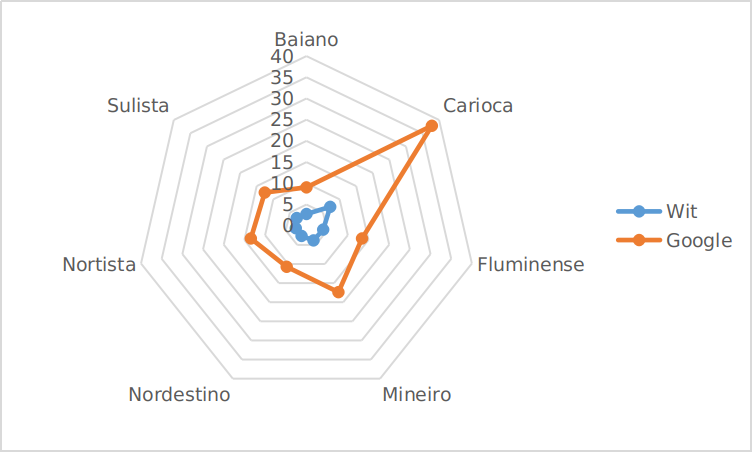
\includegraphics[width=.75\textwidth]{images/Lev_sotque_compont.png}
\fonte{elaborado pelo próprio autor (2021)}
\end{figure}

Analisando estes resultados, é possível se conjecturar que ambas as ferramentas não foram treinadas com o sotaque carioca e que este  sotaque tem características fonéticas bem diferentes, a tal ponto a prejudicar a transcrição da fala. 

\section{RESULTADO POR GÊNERO}

Nesta seção serão discutidos os resultados por gênero. O \autoref{Tabela_genero_Google_com_pontuacao} apresenta os resultados do Google Cloud considerando a pontuação para os diferentes gêneros e o \autoref{Tabela_genero_Google_sem_pontuacao} são os resultados sem considerar a pontuação. 
O \autoref{Tabela_genero_Wit_com_pontuacao} apresenta os resultados do Wit.ai considerando a pontuação para os diferentes gêneros e o \autoref{Tabela_genero_Wit_sem_pontuacao} são os resultados sem considerar a pontuação. 

Os resultados do Google Cloud são melhores para o gênero feminino que o do masculino. Nos resultados do  Wit.ai também, mas a diferença é bem pequena podendo ser considerada equiparável. 

%COM PONTUAÇÃO
\begin{quadro}[h]
\caption{Resultado do Google Cloud considerando a pontuação para análise entre gêneros} \label{Tabela_genero_Google_com_pontuacao}
\centering
\begin{tabular}{l|l|r|r|}
\hline
\multicolumn{1}{|c|}{Google Cloud}                            & Estatística   & \multicolumn{1}{l|}{Feminino} & \multicolumn{1}{l|}{Masculino} \\ \hline
\multicolumn{1}{|c|}{\multirow{2}{*}{Levenshtein}}            & Média         & \textbf{18,01}                       & 18,58                        \\ \cline{2-4} 
\multicolumn{1}{|c|}{}                                        & Mediana       & \textbf{13}                            & 15                             \\ \hline
\multicolumn{1}{|l|}{\multirow{2}{*}{\begin{tabular}[c]{@{}c@{}}Normalized \\ Levenshtein\end{tabular}}} & Média         & \textbf{89\%}                        & \textbf{89\%}                         \\ \cline{2-4} 
\multicolumn{1}{|l|}{}                                        & Mediana       & \textbf{92\%}                        & 91\%                         \\ \hline
\textbf{}                                                     & \# Acertos    & 0                             & 0                              \\ \cline{2-4} 
\textbf{}                                                     & \% de Acertos & 0\%                             & 0\%                              \\ \cline{2-4} 
\end{tabular}
\fonte{elaborado pelo próprio autor (2021)}
\end{quadro}

\begin{quadro}[h]
\caption{Resultado do Google Cloud sem considerar a pontuação para análise entre gêneros}
\label{Tabela_genero_Google_sem_pontuacao}
\centering
\begin{tabular}{l|l|r|r|}
\hline
\multicolumn{1}{|c|}{Google Cloud}                            & Estatística   & \multicolumn{1}{l|}{Feminino} & \multicolumn{1}{l|}{Masculino} \\ \hline
\multicolumn{1}{|c|}{\multirow{2}{*}{Levenshtein}}            & Média         & \textbf{13,26}                      & 13,85                       \\ \cline{2-4} 
\multicolumn{1}{|c|}{}                                        & Mediana       & \textbf{8}                             & 9                              \\ \hline
\multicolumn{1}{|l|}{\multirow{2}{*}{\begin{tabular}[c]{@{}c@{}}Normalized \\ Levenshtein\end{tabular}}} & Média         & \textbf{92\%}                      & 91\%                       \\ \cline{2-4} 
\multicolumn{1}{|l|}{}                                        & Mediana       & \textbf{95\%}                      & 94\%                        \\ \hline
\textbf{}                                                     & \# Acertos    & \textbf{80}                            & 46                             \\ \cline{2-4} 
\textbf{}                                                     & \% de Acertos & \textbf{9,36\%}                   & 5,80\%                     \\ \cline{2-4} 
\end{tabular}
\fonte{elaborado pelo próprio autor (2021)}
\end{quadro}





\begin{quadro}[h]
\caption{Resultado da Wit.ai  considerando a pontuação para análise entre gêneros} 
\label{Tabela_genero_Wit_com_pontuacao}
\centering
\begin{tabular}{l|l|r|r|}
\hline
\multicolumn{1}{|c|}{Wit.ai}                                  & Estatística   & \multicolumn{1}{l|}{Feminino} & \multicolumn{1}{l|}{Masculino} \\ \hline
\multicolumn{1}{|c|}{\multirow{2}{*}{Levenshtein}}            & Média         & \textbf{5,75}                        & 5,94                         \\ \cline{2-4} 
\multicolumn{1}{|c|}{}                                        & Mediana       & \textbf{4}                             & \textbf{4}                              \\ \hline
\multicolumn{1}{|l|}{\multirow{2}{*}{\begin{tabular}[c]{@{}c@{}}Normalized \\ Levenshtein\end{tabular}}} & Média         & \textbf{96\%}                        & \textbf{96\%}                         \\ \cline{2-4} 
\multicolumn{1}{|l|}{}                                        & Mediana       & \textbf{97\%}                        & \textbf{97\%}                         \\ \hline
\textbf{}                                                     & \# Acertos    & \textbf{51}                            & 30                             \\ \cline{2-4} 
\textbf{}                                                     & \% de Acertos & \textbf{5,97\%}                        & 3,77\%                         \\ \cline{2-4} 
\end{tabular}
\fonte{elaborado pelo próprio autor (2021) com os dados do Braccent.}
\end{quadro}

%SEM PONTUAÇÃO
\begin{quadro}[h]
\caption{Resultado da Wit.ai sem considerar a pontuação para análise entre gêneros} \label{Tabela_genero_Wit_sem_pontuacao}
\centering
\begin{tabular}{l|l|r|r|}
\hline
\multicolumn{1}{|c|}{Wit.ai}                                  & Estatística   & \multicolumn{1}{l|}{Feminino} & \multicolumn{1}{l|}{Masculino} \\ \hline
\multicolumn{1}{|c|}{\multirow{2}{*}{Levenshtein}}            & Média         & 3,22                        & \textbf{3,20}                         \\ \cline{2-4} 
\multicolumn{1}{|c|}{}                                        & Mediana       & \textbf{2}                             & \textbf{2}                              \\ \hline
\multicolumn{1}{|l|}{\multirow{2}{*}{\begin{tabular}[c]{@{}c@{}}Normalized \\ Levenshtein\end{tabular}}} & Média         & \textbf{98\%}                        & \textbf{98\%}                         \\ \cline{2-4} 
\multicolumn{1}{|l|}{}                                        & Mediana       & \textbf{98\%}                        & \textbf{98\%}                         \\ \hline
\textbf{}                                                     & \# Acertos    & \textbf{292}                           & 251                            \\ \cline{2-4} 
\textbf{}                                                     & \% de Acertos & \textbf{34,19\%}                       & 31,61\%                        \\ \cline{2-4} 
\end{tabular}
\fonte{elaborado pelo próprio autor (2021)}
\end{quadro}


\FloatBarrier

\section{RESULTADO POR GRAU DE ESCOLARIDADE}

%\todo[inline]{Thalles, ainda falta vc colocar uma tabela com o total por nível de escolaridade}

Nesta seção serão discutidos os resultados por nível de ensino. O \autoref{Tabela_ensino_Google_com_pontuacao} apresenta os resultados do Google Cloud considerando a pontuação para os diferentes níveis de ensino da pessoa e o \autoref{Tabela_Ensino_Google_sem_pontuacao} são os resultados sem considerar a pontuação. 
O \autoref{Tabela_Ensino_Wit_com_pontuacao} apresenta os resultados do Wit.ai considerando a pontuação para os diferentes níveis de ensino da pessoa  e o \autoref{Tabela_Ensino_Wit_sem_pontuacao} são os resultados sem considerar a pontuação. 



\begin{quadro}[h]
\caption{Resultado do Google Cloud  considerando a pontuação para análise entre graus de ensino (In = Incompleto, Com = Completo)}
\label{Tabela_ensino_Google_com_pontuacao}
\centering
\begin{tabular}{c|c|c|c|c|c|c|c|}
\hline
\multicolumn{1}{|c|}{\begin{tabular}[c]{@{}c@{}}Google\\ Cloud\end{tabular}}                             & Estatística  & \begin{tabular}[c]{@{}c@{}}Médio \\ In\end{tabular} & \begin{tabular}[c]{@{}c@{}}Médio \\ Com\end{tabular} & \begin{tabular}[c]{@{}c@{}}Superior \\ In\end{tabular} & \begin{tabular}[c]{@{}c@{}}Superior \\ Com\end{tabular} & Mestrado       & Doutorado \\ \hline
\multicolumn{1}{|c|}{\multirow{2}{*}{Levenshtein}}                                                       & Média        & 15,27                                               & 21,02                                                & 19,07                                                  & 18,9                                                    & \textbf{15,18} & 16,75     \\ \cline{2-8} 
\multicolumn{1}{|c|}{}                                                                                   & Mediana      & 14                                                  & 17                                                   & 15                                                     & 13                                                      & \textbf{12}    & 14        \\ \hline
\multicolumn{1}{|c|}{\multirow{2}{*}{\begin{tabular}[c]{@{}c@{}}Normalized \\ Levenshtein\end{tabular}}} & Média        & \textbf{0,91}                                       & 0,87                                                 & 0,89                                                   & 0,89                                                    & \textbf{0,91}  & 0,90      \\ \cline{2-8} 
\multicolumn{1}{|c|}{}                                                                                   & Mediana      & \textbf{0,92}                                       & 0,90                                                 & 0,90                                                   & \textbf{0,92}                                           & \textbf{0,92}  & 0,91      \\ \hline
\multicolumn{1}{l|}{}                                                                                    & \# Acertos   & 0                                                   & 0                                                    & 0                                                      & 0                                                       & 0              & 0         \\ \cline{2-8} 
\multicolumn{1}{l|}{}                                                                                    & \% de Acerto & 0                                                   & 0                                                    & 0                                                      & 0                                                       & 0              & 0         \\ \cline{2-8} 
\end{tabular}
\fonte{elaborado pelo próprio autor (2021).}
\end{quadro}

\begin{quadro}[h]
\caption{Resultado do Google Cloud sem  considerar a pontuação para análise entre graus de ensino (In = Incompleto, Com = Completo)} \label{Tabela_Ensino_Google_sem_pontuacao}
\centering
\begin{tabular}{c|c|c|c|c|c|c|c|}
\hline
\multicolumn{1}{|c|}{\begin{tabular}[c]{@{}c@{}}Google\\ Cloud\end{tabular}}                             & Estatística  & \begin{tabular}[c]{@{}c@{}}Médio \\ In\end{tabular} & \begin{tabular}[c]{@{}c@{}}Médio \\ Com\end{tabular} & \begin{tabular}[c]{@{}c@{}}Superior \\ In\end{tabular} & \begin{tabular}[c]{@{}c@{}}Superior \\ Com\end{tabular} & Mestrado      & Doutorado \\ \hline
\multicolumn{1}{|c|}{\multirow{2}{*}{Levenshtein}}                                                       & Média        & \textbf{9,86}                                       & 16,51                                                & 14,30                                                  & 14,26                                                   & 10,40         & 11,98     \\ \cline{2-8} 
\multicolumn{1}{|c|}{}                                                                                   & Mediana      & 8                                                   & 11                                                   & 10                                                     & 8                                                       & \textbf{7}    & 9         \\ \hline
\multicolumn{1}{|c|}{\multirow{2}{*}{\begin{tabular}[c]{@{}c@{}}Normalized \\ Levenshtein\end{tabular}}} & Média        & \textbf{0,94}                                       & 0,90                                                 & 0,91                                                   & 0,91                                                    & \textbf{0,94} & 0,93      \\ \cline{2-8} 
\multicolumn{1}{|c|}{}                                                                                   & Mediana      & \textbf{0,95}                                       & 0,93                                                 & 0,93                                                   & \textbf{0,95}                                           & \textbf{0,95} & 0,94      \\ \hline
\multicolumn{1}{l|}{}                                                                                    & \# Acertos   & 3                                                   & 7                                                    & 18                                                     & \textbf{65}                                             & 23            & 10        \\ \cline{2-8} 
\multicolumn{1}{l|}{}                                                                                    & \% de Acerto & 8,33                                                & 6,42                                                 & 4,60                                                   & 9,12                                                    & \textbf{9,46} & 6,36      \\ \cline{2-8} 
\end{tabular}
\fonte{elaborado pelo próprio autor (2021).}
\end{quadro}

\begin{quadro}[h]
\caption{Resultado da Wit.ai considerando a pontuação para análise entre graus de ensino (In = Incompleto, Com = Completo)} \label{Tabela_Ensino_Wit_com_pontuacao}
\centering
\begin{tabular}{c|c|c|c|c|c|c|c|}
\hline
\multicolumn{1}{|c|}{Wit.ai}                                                                            & Estatística  & \begin{tabular}[c]{@{}c@{}}Médio \\ In\end{tabular} & \begin{tabular}[c]{@{}c@{}}Médio \\ Com\end{tabular} & \begin{tabular}[c]{@{}c@{}}Superior \\ In\end{tabular} & \begin{tabular}[c]{@{}c@{}}Superior \\ Com\end{tabular} & Mestrado      & Doutorado     \\ \hline
\multicolumn{1}{|c|}{\multirow{2}{*}{Levenshtein}}                                                       & Média        & 5,13                                                        & 7,16                                                      & 7,16                                                           & 5,50                                                         & \textbf{4,72} & 5,14          \\ \cline{2-8} 
\multicolumn{1}{|c|}{}                                                                                   & Mediana      & 5                                                           & 5                                                         & 5                                                              & \textbf{4}                                                   & \textbf{4}    & \textbf{4}    \\ \hline
\multicolumn{1}{|c|}{\multirow{2}{*}{\begin{tabular}[c]{@{}c@{}}Normalized \\ Levenshtein\end{tabular}}} & Média        & \textbf{0,97}                                               & 0,95                                                      & 0,95                                                           & 0,96                                                         & \textbf{0,97} & \textbf{0,97} \\ \cline{2-8} 
\multicolumn{1}{|c|}{}                                                                                   & Mediana      & \textbf{0,97}                                               & \textbf{0,97}                                             & 0,96                                                           & \textbf{0,97}                                                & \textbf{0,97} & \textbf{0,97} \\ \hline
\multicolumn{1}{l|}{}                                                                                    & \# Acertos   & 1                                                           & 1                                                         & 12                                                             & \textbf{47}                                                  & 12            & 8             \\ \cline{2-8} 
\multicolumn{1}{l|}{}                                                                                    & \% de Acerto & 2,77                                                        & 0,91                                                      & 3,06                                                           & \textbf{6,60}                                                & 4,93          & 5,09          \\ \cline{2-8} 
\end{tabular}
\fonte{elaborado pelo próprio autor (2021).}
\end{quadro}


%SEM PONTUAÇÃO
\begin{quadro}[h]
\caption{Resultado da Wit.ai sem considerar a pontuação para análise entre graus de ensino (In = Incompleto, Com = Completo)} \label{Tabela_Ensino_Wit_sem_pontuacao}
\centering
\begin{tabular}{c|c|c|c|c|c|c|c|}
\hline
\multicolumn{1}{|c|}{Wit.ai}                                                                             & Estatística  & \begin{tabular}[c]{@{}c@{}}Médio \\ In\end{tabular} & \begin{tabular}[c]{@{}c@{}}Médio \\ Com\end{tabular} & \begin{tabular}[c]{@{}c@{}}Superior \\ In\end{tabular} & \begin{tabular}[c]{@{}c@{}}Superior \\ Com\end{tabular} & Mestrado       & Doutorado     \\ \hline
\multicolumn{1}{|c|}{\multirow{2}{*}{Levenshtein}}                                                       & Média        & \textbf{2,02}                                       & 4,55                                                 & 4,27                                                   & 3,023                                                   & 2,18           & 2,37          \\ \cline{2-8} 
\multicolumn{1}{|c|}{}                                                                                   & Mediana      & 2                                                   & 2                                                    & 2                                                      & 2                                                       & 2              & \textbf{1}    \\ \hline
\multicolumn{1}{|c|}{\multirow{2}{*}{\begin{tabular}[c]{@{}c@{}}Normalized \\ Levenshtein\end{tabular}}} & Média        & \textbf{0,98}                                       & 0,97                                                 & 0,97                                                   & \textbf{0,98}                                           & \textbf{0,98}  & \textbf{0,98} \\ \cline{2-8} 
\multicolumn{1}{|c|}{}                                                                                   & Mediana      & \textbf{0,99}                                       & 0,98                                                 & 0,98                                                   & 0,98                                                    & \textbf{0,99}  & \textbf{0,99} \\ \hline
\multicolumn{1}{l|}{}                                                                                    & \# Acertos   & 9                                                   & 26                                                   & 115                                                    & \textbf{242}                                            & 95             & 56            \\ \cline{2-8} 
\multicolumn{1}{l|}{}                                                                                    & \% de Acerto & 25                                                  & 23,85                                                & 29,41                                                  & 33,98                                                   & \textbf{39,09} & 35,66         \\ \cline{2-8} 
\end{tabular}
\fonte{elaborado pelo próprio autor (2021).}
\end{quadro}
\FloatBarrier

\begin{figure}[h!]
\centering
\caption{Gráfico em rede comparando os resultados de Levenshtein, sem considerar a pontuação, do Wit.ai e do Google Cloud, por grau de escolaridade.}
\label{fig:rede2}
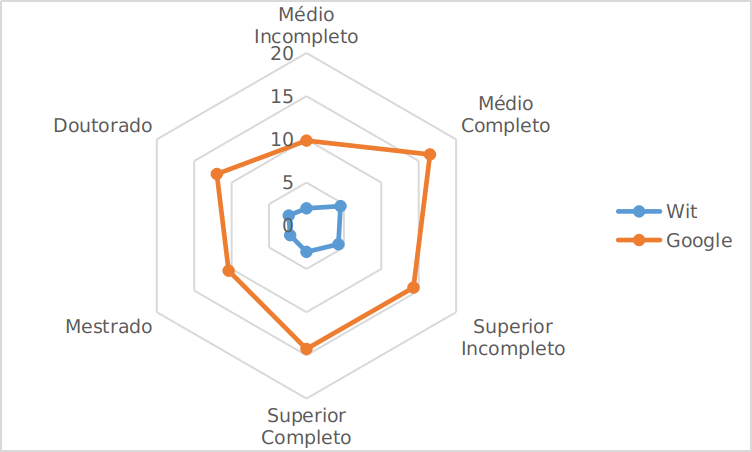
\includegraphics[width=.75\textwidth]{images/Lev_grau_sempont.png}
\fonte{elaborado pelo próprio autor (2021)}
\end{figure}

A \autoref{fig:rede2} apresenta um gráfico em rede comparando os resultados de Levenshtein, sem considerar a pontuação, em que cada ponta é um grau de escolaridade, a curva azul é o resultado do Wit.ai e a curva laranja é do Google Cloud. É possível notar que a curva de menor área é do Wit.ai, representando o melhor resultado em todos os graus de escolaridade. 
Pelos resultados, é possível verificar que o nível de ensino não é um fator discriminador para as ferramentas de transcrição considerando a base de dados usada. Se o nível de ensino fosse o fator discriminante, os valores das métricas melhorariam de acordo com o aumento do nível de ensino, e não é o que os resultados apresentam. 
%COM PONTUAÇÃO




% ----------------------------------------------------------
% Finaliza a parte no bookmark do PDF
% para que se inicie o bookmark na raiz
% e adiciona espaço de parte no Sumário
% ----------------------------------------------------------
\phantompart

% ---
% ------------------------ Conclusão ------------------------
% ---
\chapter[CONSIDERAÇÕES FINAIS]{CONSIDERAÇÕES FINAIS}

%\todo[inline]{Escreva 1 parágrafo resumo do capítulo 1, descrevendo o objetivo.}

Neste trabalho foi feito uma análise das ferramentas que realizam a transcrição de áudios. O objetivo da comparação é avaliar o nível de acurácia que cada API possui para o português do Brasil, levando em consideração também as seguintes categorias: sotaque, grau de ensino e gênero. 

%\todo[inline]{Escreva 1 parágrafo resumo do capítulo 2}

Foram selecionadas as ferramentas: Google Cloud e Wit.ai, sendo as duas de empresas consolidadas (Google e Facebook respectivamente). Ambas disponibilizam APIs de uso gratuito para a quantidade de áudios deste trabalho. Como fonte de dados foi utilizado a base Braccent, possuindo 1.648 amostras de fala divididos entre diferentes, sendo eles: nortista, baiano, fluminense, mineiro, carioca, nordestino e sulista. 

Para realizar a análise de acertos de cada ferramenta, foi utilizada a métrica de Levenshtein e a Levenshtein normalizada, que consistem em definir o menor número necessário de operações para transformar o texto transcrito para o original. O ideal seria o resultado da métrica ser igual a 0, significando  que os dois trechos são idênticos. Portanto quanto maior o resultado dessa métrica, pior é a precisão da transcrição da API, refletindo que foram necessários mais operações (inserção, exclusão ou substituição de caracteres) para transformar o trecho produzido pela ferramenta.

%\todo[inline]{Escreva 1 parágrafo resumo do capítulo 3}

Por meio da biblioteca Speech Recognition, foi feito a chamada de ambas as ferramentas para realizar a transcrição dos áudios da base. Foi observado que ao contrário da Wit.ai, o Google Cloud não faz uso de pontuação. Portanto foram realizadas duas análises, levando em consideração a pontuação e outra desconsiderando-a. 
%Com os resultados obtidos, foram gerados os valores baseados na métrica de Levenshtein para posteriormente serem analisados.


%\todo[inline]{Escreva 1 ou mais parágrafos resumo do capítulo 4}

Comparando os dados das duas APIs, é possível perceber que a Wit.ai apresenta melhores resultados que o Google Cloud. A média da métrica de Levenshtein Normalizado é de 0,96, enquanto o Google Cloud é de 0,89 considerando a pontuação. O Wit.ai acertou 81 áudios completos com pontuação. Ressalta-se que sem considerar a pontuação, essa quantidade aumenta em 6,7 vezes, acertando 543 áudios.

Na análise dos resultados por sotaque, o Google Cloud obteve melhores resultados para o sotaque baiano seguido do nordestino, e os  piores resultados foram para o sotaque carioca e não houve um único acerto para o sotaque nortista. Em todos os sotaques, o Wit.ai apresentou resultados melhores que o Google Cloud. O Wit.ai foi bem em todos os sotaques, apresentando um resultado um pouco pior para o sotaque carioca. 
Analisando estes resultados, é possível se conjecturar que ambas as ferramentas não foram treinadas com o sotaque carioca e que este sotaque tem características fonéticas bem diferentes, a tal ponto a prejudicar a transcrição da fala. 

Os resultados do Google Cloud são melhores para o gênero feminino que o do masculino. Nos resultados do  Wit.ai também, mas a diferença é bem pequena podendo ser  considerada equiparável. Quanto aos resultados por grau de escolaridade, é possível verificar que o nível de ensino não é um fator discriminador para as ferramentas de transcrição considerando a base de dados usada. Se o nível de ensino fosse o fator discriminante, os valores das métricas melhorariam de acordo com o aumento do nível de ensino, e não é o que os resultados apresentam. 

Ao final, considera-se que o Wit.ai apresentou resultados melhores em todos os cenários, além de transcrever  a pontuação.


\section{TRABALHOS FUTUROS}

Embora os objetivos propostos no trabalho tenham sido alcançados, algumas melhorias são possíveis visando trabalhos futuros:

\begin{itemize}
    \item Realizar a análise utilizando outras bases de dados de de áudios.
    \item Realizar experimentos com outros sistemas de transcrição de fala.
    \item Analisar os resultados utilizando outras métricas de comparação.
    \item Analisar e calcular a taxa de acertos por palavras. 
    
%\todo[inline]{escrever mais itens}
\end{itemize}
% ---



% ----------------------------------------------------------
% ELEMENTOS PÓS-TEXTUAIS
% ----------------------------------------------------------
\postextual
% ----------------------------------------------------------

% ----------------------------------------------------------
% Referências bibliográficas
% ----------------------------------------------------------
\renewcommand{\bibname}{REFERÊNCIAS}
\bibliography{references}

% ----------------------------------------------------------
% Glossário
% ----------------------------------------------------------
%
% Consulte o manual da classe abntex2 para orientações sobre o glossário.
%
%\glossary


% ----------------------------------------------------------
% Apêndices
% ----------------------------------------------------------

% ---
% Inicia os apêndices
% ---


%%% Início dos apêndices ---------------------------------------------
\apendices
%%% A linha abaixo impede que as seções, subseções, etc. dos apêndices e anexos
%%% sejam mostradas no Sumário.
\addtocontents{toc}{\protect\setcounter{tocdepth}{0}}

\renewcommand{\apendicesname}{APÊNDICES}
\partapendices*

% --------------------------------------------------------------------
\settocpreprocessor{chapter}{}
%\captionsbrazil

\chapter{Áudios do Braccent usados}



% Please add the following required packages to your document preamble:
% \usepackage{multirow}
\begin{table}[h]
\caption{Tabela das características dos voluntários com sotaque carioca, totalizando 81 áudios, 47 femininos e 34 masculinos.} \label{Tabela_carioca}
\begin{tabular}{|c|l|l|l|r|}
\hline
Sexo                                             & \multicolumn{1}{c|}{Grau de Escolaridade} & Cidade         & UF & \multicolumn{1}{l|}{\#} \\ \hline
\multirow{4}{*}{Feminino}                        & Ensino Superior Incompleto                & Rio de Janeiro & RJ & 15                      \\ \cline{2-5} 
                                                 & Ensino Superior Incompleto                & Rio de Janeiro & RJ & 15                      \\ \cline{2-5} 
                                                 & Mestrado                                  & Rio de Janeiro & RJ & 1                       \\ \cline{2-5} 
                                                 & Mestrado                                  & Rio de Janeiro & RJ & 16                      \\ \hline
\multicolumn{1}{|l|}{\multirow{3}{*}{Masculino}} & Ensino Superior Incompleto                & Rio de Janeiro & RJ & 16                      \\ \cline{2-5} 
\multicolumn{1}{|l|}{}                           & Ensino Superior Incompleto                & Rio de Janeiro & RJ & 3                       \\ \cline{2-5} 
\multicolumn{1}{|l|}{}                           & Ensino Superior Incompleto                & Rio de Janeiro & RJ & 15                      \\ \hline
\end{tabular}
\fonte{elaborado pelo próprio autor (2021) com os dados do Braccent.}

\end{table}

% Please add the following required packages to your document preamble:
% \usepackage{multirow}
\begin{table}[h]
\caption{Tabela das características dos voluntários com sotaque mineiro, totalizando 137 áudios, 58 femininos e 79 masculinos.} \label{Tabela_mineiro}
\begin{tabular}{|l|l|l|l|l|}
\hline
\multicolumn{1}{|c|}{Sexo} & \multicolumn{1}{c|}{Grau de Escolaridade} & Cidade         & UF & \# \\ \hline
\multirow{7}{*}{Feminino}  & Ensino Superior Incompleto                & Araxá          & MG & 12 \\ \cline{2-5} 
                           & Mestrado                                  & Uberaba        & MG & 13 \\ \cline{2-5} 
                           & Ensino Superior Incompleto                & Araxá          & MG & 6  \\ \cline{2-5} 
                           & Ensino Superior Incompleto                & Viçosa         & MG & 5  \\ \cline{2-5} 
                           & Doutorado                                 & Viçosa         & MG & 3  \\ \cline{2-5} 
                           & Doutorado                                 & Belo Horizonte & MG & 11 \\ \cline{2-5} 
                           & Mestrado                                  & Belo Horizonte & MG & 8  \\ \hline
\multirow{6}{*}{Masculino} & Ensino Superior Incompleto                & Belo Horizonte & MG & 14 \\ \cline{2-5} 
                           & Ensino Superior Completo                  & Belo Horizonte & MG & 15 \\ \cline{2-5} 
                           & Ensino Superior Completo                  & Belo Horizonte & MG & 16 \\ \cline{2-5} 
                           & Ensino Superior Completo                  & Belo Horizonte & MG & 16 \\ \cline{2-5} 
                           & Ensino Superior Completo                  & Pato de Minas  & MG & 15 \\ \cline{2-5} 
                           & Ensino Superior Completo                  & Juiz de Fora   & MG & 3  \\ \hline
\end{tabular}
\fonte{elaborado pelo próprio autor (2021) com os dados do Braccent.}
\end{table}

% Please add the following required packages to your document preamble:
% \usepackage{multirow}
\begin{table}[h]
\caption{Tabela das características dos voluntários com sotaque fluminense, totalizando 110 áudios, 61 femininos e 49 masculinos.} \label{Tabela_fluminense}
\begin{tabular}{|l|l|l|l|r|}
\hline
\multicolumn{1}{|c|}{Sexo} & \multicolumn{1}{c|}{Grau de Escolaridade} & Cidade              & UF & \multicolumn{1}{l|}{\#} \\ \hline
\multirow{6}{*}{Feminino}  & Mestrado                                  & São Mateus          & ES & 15                      \\ \cline{2-5} 
                           & Mestrado                                  & Ubatuba             & SP & 4                       \\ \cline{2-5} 
                           & Ensino Superior Completo                  & São Mateus          & ES & 16                      \\ \cline{2-5} 
                           & Ensino Superior Incompleto                & Cariacica           & ES & 14                      \\ \cline{2-5} 
                           & Ensino Superior Completo                  & Campo de Goytacazes & RJ & 10                      \\ \cline{2-5} 
                           & Ensino Superior Incompleto                & Vitória             & ES & 2                       \\ \hline
\multirow{4}{*}{Masculino} & Ensino Superior Incompleto                & Cariacica           & ES & 13                      \\ \cline{2-5} 
                           & Ensino Superior Completo                  & Viana               & ES & 14                      \\ \cline{2-5} 
                           & Ensino Superior Completo                  & Linhares            & ES & 10                      \\ \cline{2-5} 
                           & Ensino Superior Completo                  & Aracruz             & ES & 12                      \\ \hline
\end{tabular}
\fonte{elaborado pelo próprio autor (2021) com os dados do Braccent.}
\end{table}

% Please add the following required packages to your document preamble:
% \usepackage{multirow}
% \usepackage[table,xcdraw]{xcolor}
% If you use beamer only pass "xcolor=table" option, i.e. \documentclass[xcolor=table]{beamer}
\begin{table}[h]
\caption{Tabela das características dos voluntários com sotaque baiano, totalizando 173 áudios, 99 femininos e 74 masculinos.} \label{Tabela_baiano}
\begin{tabular}{|l|l|l|l|l|}
\hline
\multicolumn{1}{|c|}{Sexo}  & \multicolumn{1}{c|}{Grau de Escolaridade} & Cidade           & UF & \multicolumn{1}{r|}{\#}    \\ \hline
\multirow{7}{*}{Feminino}
                            &             Ensino Superior Completo                  & Aracaju          & SE & 15 \\ \cline{2-5} 
                            &           Doutorado                                 & Brumado          & BA & 16                         \\ \cline{2-5} 
                            &              Ensino Superior Incompleto                & Salvador         & BA & 7                          \\ \cline{2-5} 
                            &                   Ensino Médio Completo                     & Salvador         & BA & 15                         \\ \cline{2-5} 
                            &                  Ensino Superior Completo                  & Ilheus           & BA & 15                         \\ \cline{2-5} 
                            &     Ensino Superior Incompleto                & Montes Claros    & MG & 16                         \\ \cline{2-5} 
\multirow{8}{*}{Masculino}    & Mestrado                                  & Salvador         & BA & 15                         \\ \hline
                                           & Ensino Superior Incompleto                & Montes Claros    & MG & 16                         \\ \cline{2-5} 
                             & Doutorado                                 & Aracaju          & SE & 12                         \\ \cline{2-5} 
                    & Mestrado                                  & São Francisco    & MG & 15                         \\ \cline{2-5} 
                           & Ensino Superior Incompleto                & Ipiau            & BA & 1                          \\ \cline{2-5} 
                         & Ensino Superior Incompleto                & Salvador         & BA & 7                          \\ \cline{2-5} 
                          & Ensino Médio Completo                     & Salvador         & BA & 8                          \\ \cline{2-5} 
                         & Ensino Superior Completo                  & Simões Filho     & BA & 2                          \\ \cline{2-5} 
  & Ensino Médio Completo                     & Feira de Santana & BA & 13                         \\ \hline
\end{tabular}
\fonte{elaborado pelo próprio autor (2021) com os dados do Braccent.}
\end{table}


\begin{table}[h]
\caption{Tabela das características dos voluntários com sotaque nortista, totalizando 24 áudios, 6 femininos e 18 masculinos.} \label{Tabela_nortista}
\begin{tabular}{|c|l|l|l|l|}
\hline
Sexo                       & Grau de Escolaridade       & Cidade    & UF & \# \\ \hline
Feminino                   & Ensino Superior Incompleto & Belém     & PA & 6  \\ \hline
\multirow{2}{*}{Masculino} & Mestrado                   & Palmas    & TO & 4  \\ \cline{2-5} 
                           & Mestrado                   & Parintins & AM & 14 \\ \hline
\end{tabular}
\fonte{elaborado pelo próprio autor (2021) com os dados do Braccent.}
\end{table}


\begin{table}[h]
\caption{Tabela das características dos voluntários com sotaque nordestino, totalizando 333 áudios, 158 femininos e 175 masculinos.} \label{Tabela_sulist}
\begin{tabular}{|l|l|l|l|r|}
\hline
\multicolumn{1}{|c|}{Sexo}   & \multicolumn{1}{c|}{Grau de Escolaridade}     & Cidade            & UF & \multicolumn{1}{l|}{\#} \\ \hline
                             & Ensino Superior Incompleto                    & Campina Grande    & PB & 2                       \\ \cline{2-5} 
                             & Ensino Superior Completo                      & Fortaleza         & CE & 16                      \\ \cline{2-5} 
                             & Ensino Superior Completo                      & Paulo Afonso      & BA & 15                      \\ \cline{2-5} 
                             & Ensino Superior Completo                      & Paulo Afonso      & BA & 16                      \\ \cline{2-5} 
                             & Ensino Superior Completo                      & Paulo Afonso      & BA & 16                      \\ \cline{2-5} 
                             & Ensino Superior Incompleto                    & Campina Grande    & PB & 16                      \\ \cline{2-5} 
                             & Ensino Superior Completo                      & Paulo Afonso      & BA & 14                      \\ \cline{2-5} 
                             & Ensino Superior Completo                      & Campina Grande    & PB & 16                      \\ \cline{2-5} 
                             & Ensino Superior Completo                      & Paulo Afonso      & BA & 3                       \\ \cline{2-5} 
                             & Ensino Superior Completo                      & Campina Grande    & PB & 6                       \\ \cline{2-5} 
                             & Ensino Médio Incompleto                       & Paulo Afonso      & BA & 15                      \\ \cline{2-5} 
                             & Doutorado                                     & Campina Grande    & PB & 16                      \\ \cline{2-5} 
\multirow{-13}{*}{Feminino}  & Ensino Superior Completo                      & Paulo Afonso      & BA & 10                      \\ \hline
                             & Ensino Superior Completo                      & Juazeiro do Norte & CE & 15                      \\ \cline{2-5} 
                             & Doutorado                                     & Campina Grande    & PB & 9                      \\ \cline{2-5} 
                             & Ensino Superior Completo                      & Fortaleza         & CE & 4                       \\ \cline{2-5} 
                             & Ensino Superior Incompleto                    & Campina Grande    & PB & 15                      \\ \cline{2-5} 
                             & Mestrado                                      & Natal             & RN & 15                      \\ \cline{2-5} 
                             & Ensino Superior Completo                      & Fortaleza         & CE & 7                      \\ \cline{2-5} 
                             & Doutorado                                     & Imperatriz        & MA & 16                      \\ \cline{2-5} 
                             & Ensino Superior Completo                      & Paulo Afonso      & BA & 15                      \\ \cline{2-5}
                             & Mestrado                                      & Maceió            & AL & 13                      \\ \cline{2-5} 
                             & Mestrado                                      & Pesqueira         & PE & 12                      \\ \cline{2-5} 
                             & Ensino Superior Completo                      & Paulo Afonso      & BA & 14                      \\ \cline{2-5} 
                             & Ensino Superior Completo                      & Paulo Afonso      & BA & 1                       \\ \cline{2-5} 
                             & Ensino Superior Completo                      & Campina Grande    & PB & 7                       \\ \cline{2-5} 
                             & Ensino Superior Completo                      & Paulo Afonso      & BA & 16                      \\ \cline{2-5} 
                             & Mestrado                                      & Campina Grande    & PB & 3                       \\ \cline{2-5} 
                             & Ensino Superior Incompleto                    & Campina Grande    & PB & 10                      \\ \cline{2-5} 
\multirow{-18}{*}{Masculino} & Ensino médio completo & Paulo Afonso      & BA & 3                       \\ \hline
\end{tabular}
\fonte{elaborado pelo próprio autor (2021) com os dados do Braccent.}
\end{table}

% Please add the following required packages to your document preamble:
% \usepackage{multirow}
\begin{table}[h]
\caption{Tabela das características dos voluntários com sotaque sulista, totalizando 790 áudios, sendo 425 femininos.} \label{Tabela_sulista_fem}

\begin{tabular}{|l|l|l|l|r|}
\hline
\multicolumn{1}{|c|}{Sexo} & \multicolumn{1}{c|}{Grau de Escolaridade} & Cidade              & UF & \multicolumn{1}{l|}{\#} \\ \hline
\multirow{32}{*}{Feminino} & Ensino Superior Completo                  & São Paulo           & SP & 15                      \\ \cline{2-5} 
                           & Ensino Superior Completo                  & Paulinia            & SP & 6                       \\ \cline{2-5} 
                           & Ensino Superior Completo                  & São Paulo           & SP & 16                      \\ \cline{2-5} 
                           & Ensino Superior Completo                  & Campinas            & SP & 15                      \\ \cline{2-5} 
                           & Ensino Superior Completo                  & Paraisópolis        & MG & 16                      \\ \cline{2-5} 
                           & Ensino Superior Incompleto                & São Paulo           & SP & 7                       \\ \cline{2-5} 
                           & Ensino Superior Completo                  & São José dos Campos & SP & 16                      \\ \cline{2-5} 
                           & Ensino Superior Completo                  & Ribeirão Preto      & SP & 16                      \\ \cline{2-5} 
                           & Mestrado                                  & Bragança Paulista   & SP & 16                      \\ \cline{2-5} 
                           & Ensino Superior Incompleto                & Valinhos            & SP & 16                      \\ \cline{2-5} 
                           & Ensino Superior Incompleto                & São Paulo           & SP & 15                      \\ \cline{2-5} 
                           & Ensino Superior Completo                  & Campinas            & SP & 2                       \\ \cline{2-5} 
                           & Mestrado                                  & Estrela             & RS & 16                      \\ \cline{2-5} 
                           & Ensino Superior Completo                  & São Paulo           & SP & 14                      \\ \cline{2-5} 
                           & Ensino Superior Incompleto                & Navegantes          & SC & 16                      \\ \cline{2-5} 
                           & Ensino Superior Incompleto                & Cabo Verde          & MG & 1                       \\ \cline{2-5} 
                           & Ensino Superior Incompleto                & Salto               & SP & 15                      \\ \cline{2-5} 
                           & Ensino Superior Incompleto                & Guarulhos           & SP & 15                      \\ \cline{2-5} 
                           & Mestrado                                  & Passos              & MG & 15                      \\ \cline{2-5} 
                           & Ensino Superior Completo                  & Indaiatuba          & SP & 16                      \\ \cline{2-5} 
                           & Doutorado                                 & São Paulo           & SP & 16                      \\ \cline{2-5} 
                           & Ensino Médio Completo                     & Campinas            & SP & 15                      \\ \cline{2-5} 
                           & Ensino Superior Completo                  & Campinas            & SP & 15                      \\ \cline{2-5} 
                           & Ensino Superior Incompleto                & São Paulo           & SP & 15                      \\ \cline{2-5} 
                           & Ensino Superior Completo                  & Goiânia             & GO & 16                      \\ \cline{2-5} 
                           & Ensino Superior Incompleto                & Campinas            & SP & 16                      \\ \cline{2-5} 
                           & Ensino Superior Completo                  & Campinas            & SP & 5                       \\ \cline{2-5} 
                           & Ensino Superior Completo                  & Piracicaba          & SP & 16                      \\ \cline{2-5} 
                           & Ensino Superior Completo                  & Poços de Caldas     & SP & 15                      \\ \cline{2-5} 
                           & Ensino Superior Completo                  & Poços de Caldas     & SP & 15                      \\ \cline{2-5} 
                           & Ensino Superior Incompleto                & São Paulo           & SP & 1                       \\ \cline{2-5} 
                           & Mestrado                                  & Limeira             & SP & 16                      \\ \hline
\end{tabular}
\fonte{elaborado pelo próprio autor (2021) com os dados do Braccent.}
\end{table}


% Please add the following required packages to your document preamble:
% \usepackage{multirow}
% \usepackage[table,xcdraw]{xcolor}
% If you use beamer only pass "xcolor=table" option, i.e. \documentclass[xcolor=table]{beamer}
% \usepackage[normalem]{ulem}
% \useunder{\uline}{\ul}{}
\begin{table}[h]
\caption{Tabela das características dos voluntários com sotaque sulista, totalizando 790 áudios, sendo 365 masculinos.} \label{Tabela_sulista_fem}

\begin{tabular}{|l|l|l|l|r|}
\hline
Sexo                         & Grau de escolaridade           & Cidade              & UF & \multicolumn{1}{l|}{\#} \\ \hline
                             & Mestrado                       & Campinas            & SP & 16                      \\ \cline{2-5} 
                             & Ensino Superior Incompleto     & São Paulo           & SP & 1                       \\ \cline{2-5} 
                             & Doutorado                      & Limeira             & SP & 13                      \\ \cline{2-5} 
                             & Ensino Superior Incompleto     & Curitiba            & PR & 1                       \\ \cline{2-5} 
                             & Ensino Superior Incompleto     & Itu                 & SP & 11                      \\ \cline{2-5} 
                             & Ensino Superior Incompleto     & São José dos Campos & SP & 16                      \\ \cline{2-5} 
                             & Doutorado                      & Pederneiras         & SP & 16                      \\ \cline{2-5} 
                             & Ensino Superior Completo       & São Paulo           & SP & 16                      \\ \cline{2-5} 
                             & Ensino Médio Completo          & Ribeirão Preto      & SP & 12                      \\ \cline{2-5} 
                             & Ensino Superior Completo       & São Paulo           & SP & 16                      \\ \cline{2-5} 
                             & Ensino Superior Incompleto     & Santo André         & SP & 15                      \\ \cline{2-5} 
                             & Ensino Superior Completo       & São Paulo           & SP & 16                      \\ \cline{2-5} 
                             & Ensino Superior Completo       & Assis               & SP & 15                      \\ \cline{2-5} 
                             & Ensino Superior Incompleto     & São Paulo           & SP & 4                       \\ \cline{2-5} 
                             & Ensino Superior Completo       & Porto Alegre        & RS & 3                       \\ \cline{2-5} 
                             & Ensino Superior Incompleto     & Tatuí               & SP & 9                      \\ \cline{2-5} 
                             & Ensino Superior Completo       & Bauru               & SP & 16                      \\ \cline{2-5} 
                             & Ensino Superior Completo       & Piracicaba          & SP & 14                      \\ \cline{2-5} 
                             & Ensino Superior Incompleto     & Campo Grande        & MS & 15                      \\ \cline{2-5} 
                             & Ensino Superior Completo       & Botucatu            & SP & 16                      \\ \cline{2-5} 
                             & Ensino Superior Incompleto     & Goiânia             & GO & 4                       \\ \cline{2-5} 
                             & Ensino Médio Completo          & São José dos Campos & SP & 11                      \\ \cline{2-5} 
                             & Ensino Superior Completo       & Palmital            & SP & 15                      \\ \cline{2-5} 
                             & Ensino Superior Completo       & Cachoeira do Sul    & RS & 14                      \\ \cline{2-5} 
                             & Ensino Médio Incompleto        & Caixas do Sul       & RS & 5                       \\ \cline{2-5} 
                             & Ensino Médio Completo          & São Paulo           & SP & 1                       \\ \cline{2-5} 
                             & Doutorado                      & Limeira             & SP & 16                      \\ \cline{2-5} 
                             & Ensino Superior Completo       & Campinas            & SP & 13                      \\ \cline{2-5} 
                             & Ensino Médio Completo          & Curitiba            & PR & 13                      \\ \cline{2-5} 
                             & Mestrado                       & Brasília            & DF & 14                      \\ \cline{2-5} 
                             & Doutorado & Porto Alegre        & RS & 13                      \\ \cline{2-5} 
\multirow{-32}{*}{Masculino} & Ensino Médio Incompleto        & Curitiba            & PR & 5                       \\ \hline
\end{tabular}
\fonte{elaborado pelo próprio autor (2021) com os dados do Braccent.}
\end{table}




%---------------------------------------------------------------------
% INDICE REMISSIVO
%---------------------------------------------------------------------
\phantompart

%---------------------------------------------------------------------

\end{document}